
%%%%%%%%%%%%%%%%%%%%%%%%%%%%%%%%%%%%%%%%%%%%%%%%%%%%%%%%%%%%%%%%%%%%
%% I, the copyright holder of this work, release this work into the
%% public domain. This applies worldwide. In some countries this may
%% not be legally possible; if so: I grant anyone the right to use
%% this work for any purpose, without any conditions, unless such
%% conditions are required by law.
%%%%%%%%%%%%%%%%%%%%%%%%%%%%%%%%%%%%%%%%%%%%%%%%%%%%%%%%%%%%%%%%%%%%

\documentclass[compress]{beamer}
\usetheme[faculty=phil, navigation, microtype]{fibeamer}
%\usetheme[logo=resources/NOKIA]{fibeamer}
\useoutertheme{miniframes}
\setbeamercolor{section in head/foot}{fg=white, bg=fibeamer@blue}
\usepackage[francais]{babel}
\usepackage[utf8]{inputenc}
\usepackage[T1]{fontenc}
%\title{Requêtes probabilistes et pondérées en logique d'arbre de calcul %
\includegraphics[width=0.25\linewidth]{fibeamer/logo/mu/storm}
\title{Synthèse Multi-objectifs dans les Processus Décisionnels de Markov} %% that will be typeset on the
%\subtitle{Presentation Subtitle} %% title page.
\author{Florent Delgrange}
\vspace{0.5cm}
\subtitle{\normalsize Mab2 Sciences Informatiques}
\date{\today}
%% These additional packages are used within the document:
\usepackage{ragged2e}  % `\justifying` text
\usepackage{cancel}
\usepackage{bbold}
\usepackage{booktabs}  % Tables
\usepackage{slashed}
\usepackage{centernot}
\usepackage{tabularx}
\usepackage{tikz}      % Diagrams
\usetikzlibrary{calc, shapes, backgrounds}
\usepackage{arevtext,arevmath}
\usepackage{verbatim}
\usepackage{amsmath, amssymb}
\usepackage{url}       % `\url`s
\usepackage{listings}
\usepackage{changepage}
\usepackage{cprotect}
\usepackage{caption}
\usepackage{graphicx}
\usepackage{minted}
\usepackage{biblatex}
\usepackage{mathtools}
\usepackage{multicol}
\usepackage{bbold}
\usepackage{cancel}
\usepackage{hhline}
\frenchspacing

\newcommand\TS{\text{\sffamily TS}}
\newcommand{\STAB}[1]{\begin{tabular}{@{}c@{}}#1\end{tabular}}

\newenvironment{proenv}{\only{\setbeamercolor{local structure}{fg=lightgray}}}{}

%% PRISM CODE LISTING *********************************************

\definecolor{prismgreen}{rgb}{0, 0.6, 0}

\lstdefinelanguage{Prism}{ % syntax highlight via font
	basicstyle=\color{red}\tiny\ttfamily, % small true type font (like courier)
	keywords=
	{bool,C,ceil,const,ctmc,double,dtmc,endinit,endmodule,endrewards, endsystem,F,false,floor,formula,G,global,I,init,int,label,max,mdp,min,
	module,nondeterministic,P,Pmin,Pmax,prob,probabilistic,R,rate,rewards, Rmin,Rmax,S,stochastic,system,true,U,X},
	keywordstyle={\bfseries\color{black}},
	numberstyle=\tiny\color{black},
	comment=[l] {//}, morecomment=[s]{/*}{*/}, % single and multi-line
	commentstyle= \color{prismgreen}, % dark green
	tabsize=4, % tab treatment (going to be fixed in Prism)
	captionpos=b, % put captions at the bottom
	escapechar=@ % write LaTeX comments escaped by @ symbol
}

%define command \prism with one argument for inline printing of \prism code
\newcommand{\prism}[1]{\lstinline[language=Prism,basicstyle=\small
	\ttfamily]|#1|}

%% END PRISM CODE LISTING


\definecolor{DarkOrange}{HTML}{FF8C00}
\theoremstyle{theorem}%{3pt}{3pt}{\slshape}{}{\bfseries}{.}{.5em}{}
\newtheorem{theoreme}{Théorème}
\newtheorem{lemme}{Lemme}
\newtheorem{exemple}{Exemple}


\newcommand\sfont[1]{\textnormal{\fontfamily{qpl}\selectfont #1}}

\bibliography{bib}
\begin{document}
  \begin{frame}[plain]
    \maketitle
    \vspace{.05\linewidth}
    \begin{columns}
      \begin{column}{0.5\linewidth}
        
\includegraphics[width=0.55\linewidth]{UMONS+txt_white}
      \end{column}
      \begin{column}{0.5\linewidth}
        \flushright
        \vspace{-.02\linewidth}
        
\includegraphics[width=0.5\linewidth]{UMONS_FS_white}
      \end{column}
    \end{columns}
    \begin{center}
      \color{white}
      \bfseries
      Année académique 2017-2018
    \end{center}
  \end{frame}


% \AtBeginSection[]
%   {
%     %  \begin{frame}<beamer>
%     %  \frametitle{Plan}
%     %  \tableofcontents[currentsection]
%     %  \end{frame}
%     \begin{frame}{\contentsname}
%     \footnotesize
%     \vspace{-0.05\linewidth}
%     %\footnotesize
%     %\begin{multicols}{2}
%     \tableofcontents[currentsection]
%     %\end{multicols}
%
%     \end{frame}
%   }

\section{Contexte}

\subsection{Vérification formelle et synthèse de stratégie : motivations}
\begin{frame}{Vérification et synthèse}\footnotesize
  %\vspace{-.03\linewidth}
  \begin{itemize}
    \item Systèmes réactifs dans des environnements stochastiques
    \begin{itemize}
      \footnotesize
      \item[$\rightarrow$] \textit{exemples} : protocoles de communication, réseaux de capteurs, voitures autonomes, etc.
    \end{itemize}
    \item[-] \textbf{\color{fibeamer@orange}Vérification} de l'\textbf{\color{fibeamer@orange}exactitude} du comportement de tels systèmes \item[-]\textbf{\color{orange}Synthèse} de \textbf{\color{orange}stratégies} satisfaisant des \textbf{\color{orange}objectifs} dans de tels systèmes
    \begin{itemize}
      \footnotesize
      \item[$\rightarrow$] \alert{\textbf{Décisif !}}
      \item absence de bugs
      \item \alert{sécurité}
    \end{itemize}
    %\item[$\rightarrow$] \textbf{\color{fibeamer@orange}Synthétiser} automatiquement des \textbf{\color{fibeamer@orange}stratégies} optimales
  \end{itemize}
  \begin{center}
  \vspace{-.03\linewidth}
  \begin{columns}
    \begin{column}{0.5\linewidth}
    \begin{figure}
      \centering
      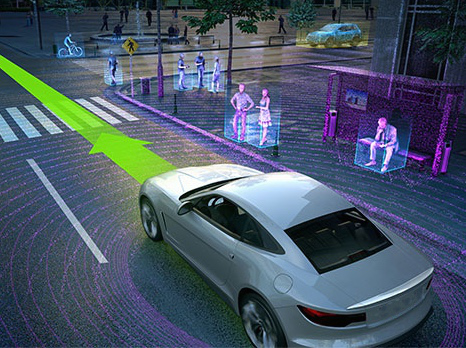
\includegraphics[width=0.7\linewidth]{resources/autonomous-cars}
    \end{figure}
    \end{column}
    \begin{column}{0.5\linewidth}
    \begin{figure}
      \centering
      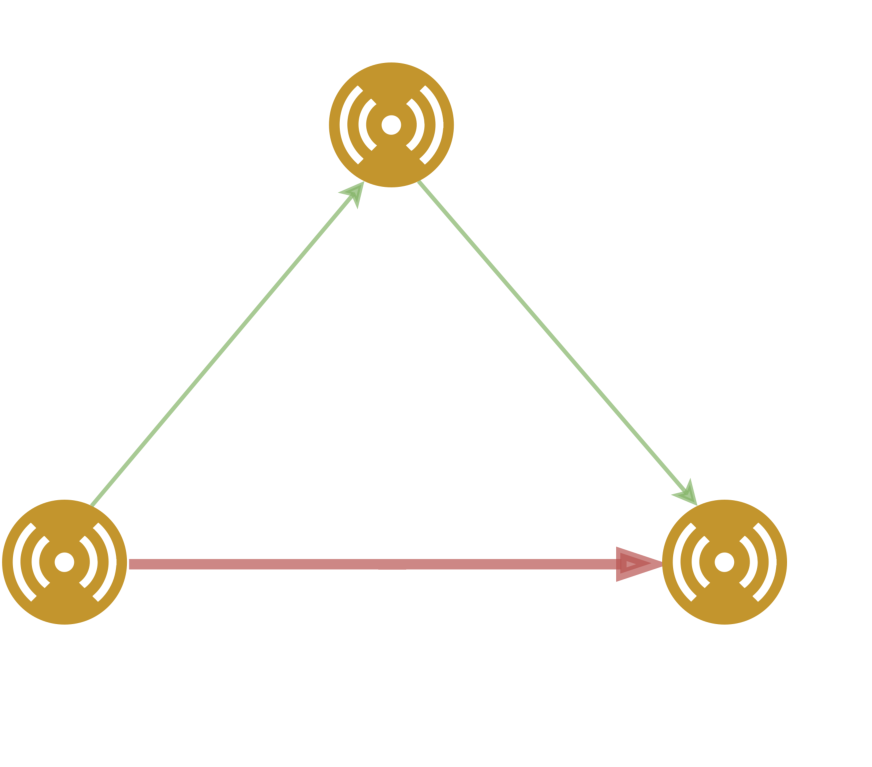
\includegraphics[width=0.7\linewidth]{resources/example3.pdf}
    \end{figure}
    \end{column}
  \end{columns}

  \end{center}
\end{frame}

\begin{frame}{Vérification formelle}\small
  \begin{itemize}
    \item Le \textit{testing} démontre la présence de bugs, mais pas leur absence !
    \item Les algorithmes de \textit{\color{orange}model-checking} permettent d'automatiquement \textbf{\color{fibeamer@orange}vérifier formellement} des \textit{\color{fibeamer@orange}propriétés} dans un système
    \end{itemize}
    \begin{center}
      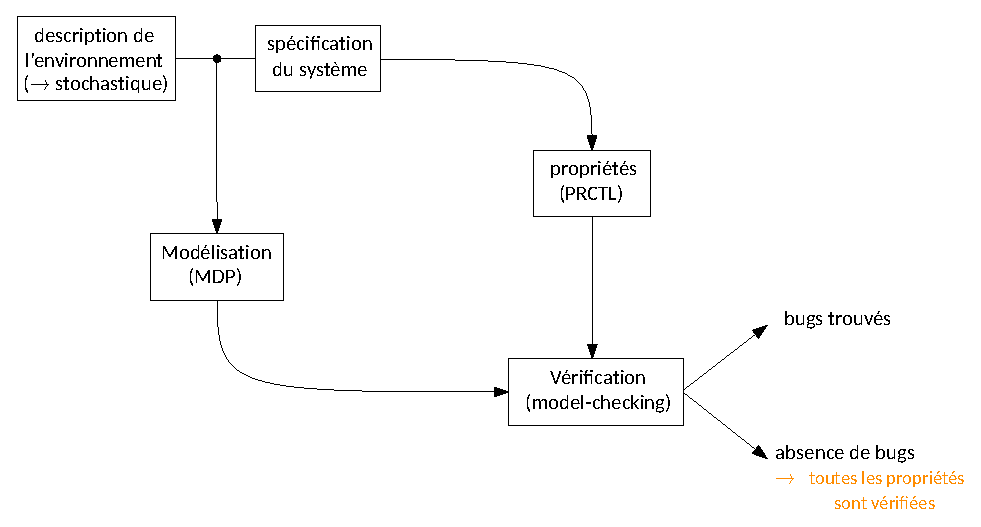
\includegraphics[width=0.9\linewidth]{resources/formal-verif}
    \end{center}
  %   \item des logiques permettent d'exprimer ces propriétés
  %   \item[$\leadsto$] pour les MDPs avec une fonction de coût: \textbf{\color{fibeamer@orange}PRCTL}
  %   \begin{itemize}
  %     \item[$\rightarrow$] permet d'exprimer des propriétés d'\textit{\color{fibeamer@orange}accessibilité}, de \textit{\color{fibeamer@orange}persistance}, d'\textit{\color{fibeamer@orange}accessibilité répétée} tout en considérant le coût des décisions
  %   \end{itemize}
\end{frame}


\begin{frame}{Synthèse de stratégie}
  \begin{itemize}
    \item Construire la stratégie satisfaisant un problème dans le système
  \end{itemize}
  \begin{center}
    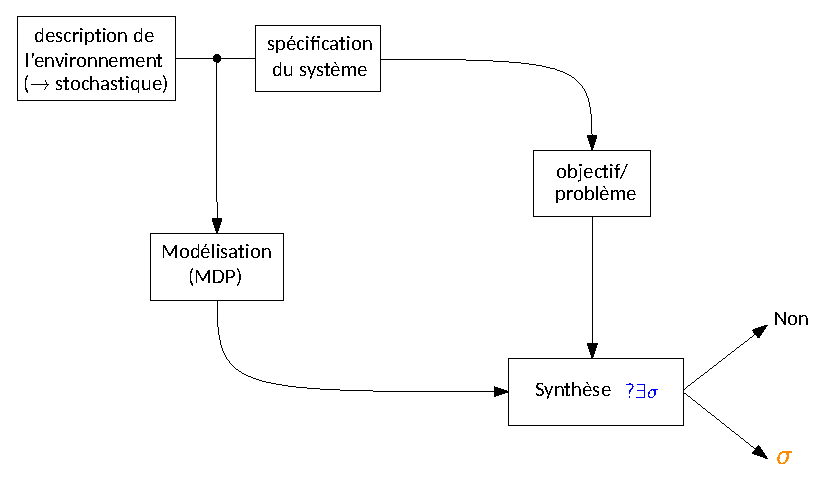
\includegraphics[width=0.83\linewidth]{resources/synthese}
  \end{center}
\end{frame}

\subsection{But}

\begin{frame}{But du mémoire} \footnotesize
  \begin{itemize}
    \item Synthèse de \textbf{\color{fibeamer@orange}stratégies} satisfaisant des problèmes \textbf{\color{fibeamer@orange}mono-objectifs} de \textbf{\color{fibeamer@orange}plus court chemin stochastique}
    \item Synthèse de \textbf{\color{orange}stratégies} satisfaisant \textbf{\itshape \color{fibeamer@orange}simultanément} plusieurs objectifs en
    milieu \textbf{\color{fibeamer@orange}stochastique}
    \item \'Etudier \textbf{\itshape\color{fibeamer@blue}PRCTL}, une logique permettant d'\textbf{\color{fibeamer@orange}exprimer des propriétés} %pour la \textbf{\color{fibeamer@orange}vérification de modèles probabilistes}
    pour les modèles probabilistes
    ainsi que ses algorithmes de \textbf{\color{fibeamer@orange}model-checking}
    \item Apporter une contribution à \sfont{\color{fibeamer@orange}Storm}
  \end{itemize}
    \begin{columns}
      \begin{column}{0.55\linewidth}
        \vspace{-.05\linewidth}
        \begin{itemize}\footnotesize
            \item[$\leadsto$] Model-checker probabiliste en développement
            \item[$\leadsto$] Implémente des algorithmes récents de model-checking multi-objectif
            \item[$\leadsto$] \'Etude de l'outil (algorithmes, articles, etc.)
            %\item[$\leadsto$] Université de Aachen
        \end{itemize}
      \end{column}
      \begin{column}{0.2\linewidth}
          
\includegraphics[width=\linewidth]{resources/storm}\\
          
\includegraphics[width=\linewidth]{resources/rwth}
      \end{column}
    \end{columns}
\end{frame}

\section{Processus décisionnels de Markov}
\subsection{Définition}
\begin{frame}{Processus décisionnel de Markov (MDP)}\small
% \begin{figure}
%   \centering
  \begin{overprint}

    \onslide<1>\centerline{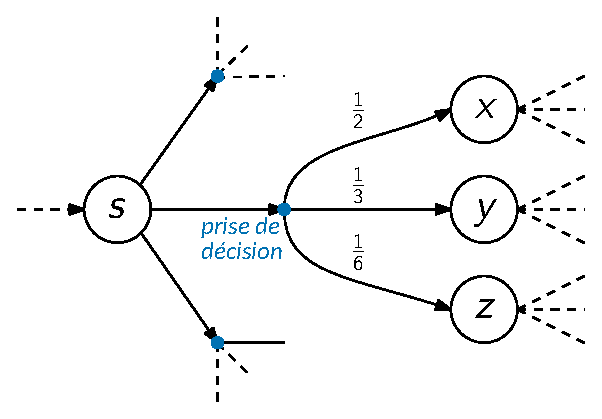
\includegraphics[width=0.45\linewidth]{resources/PDMintro}}
    \onslide<2>\centerline{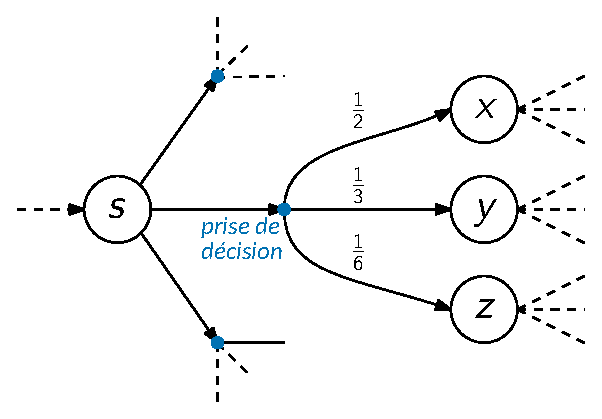
\includegraphics[width=0.45\linewidth]{resources/PDMintro}}
    \onslide<3>\centerline{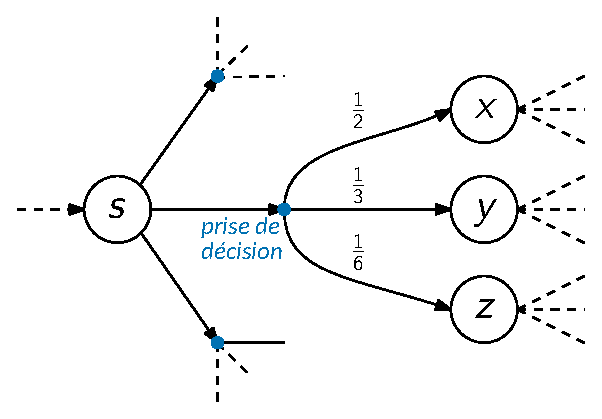
\includegraphics[width=0.45\linewidth]{resources/PDMintro}}
    \onslide<4>\centerline{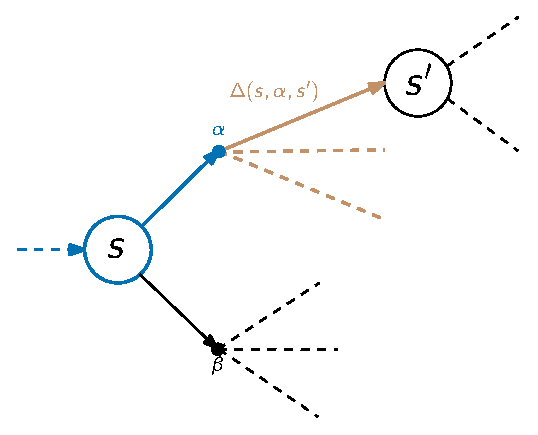
\includegraphics[width=0.45\linewidth]{resources/go1}}
    \onslide<5>\centerline{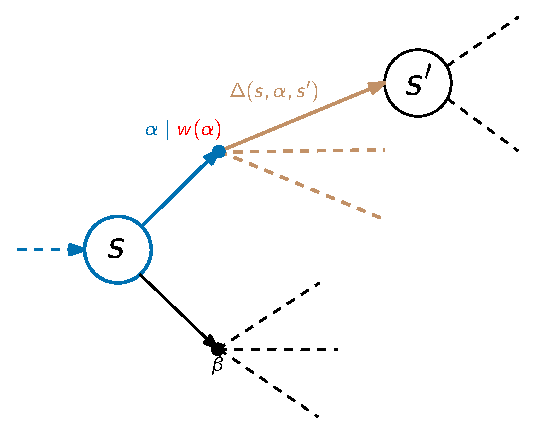
\includegraphics[width=0.45\linewidth]{resources/go2}}
    \onslide<6>\centerline{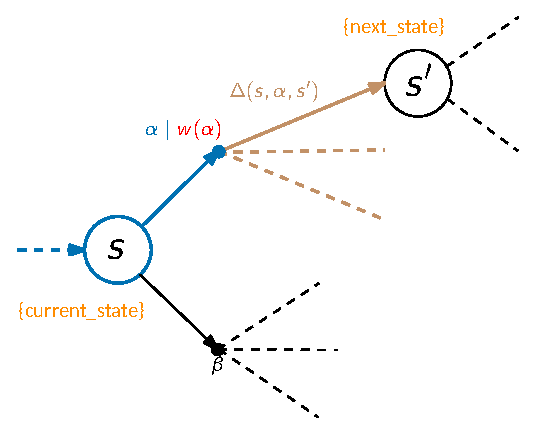
\includegraphics[width=0.45\linewidth]{resources/go3}}
  \end{overprint}
%  \end{figure}
  \only<1>{
  %\vspace{-.05\linewidth}
    \begin{itemize}
      \item \textit{Système \textbf{\color{fibeamer@orange}stochastique}}
      \item permet de modéliser à la fois des \textbf{\color{fibeamer@orange}situations probabilistes} et \textbf{\color{fibeamer@orange}non-déterministes} (i.e., nécessitant des prises de décision)
      \item peut être enrichi avec une \textbf{\color{fibeamer@orange}fonction de poids}, permettant de pondérer le \textbf{\color{fibeamer@orange}coût} de chaque décision
    \end{itemize}
    }
    \only<2->{
    \footnotesize
    %Un MDP est un tuple $\mathcal{M} = (S, A, \Delta, w, AP, L)$ où
    %\vspace{-.04\linewidth}
  \begin{itemize}
    \item<2-> {\color{fibeamer@blue}$S$} est un ensemble fini d'états et {\color{fibeamer@blue}$A$} est un ensemble fini d'actions,
    \begin{itemize}\footnotesize
      \item<2->[$\rightarrow$] $\forall s \in S, \;$ $\color{fibeamer@blue} A(s) \subseteq A$ est l'ensemble des \textit{\color{fibeamer@orange} actions activées } de $s$,
    \end{itemize}
    \item<3-> {\color{fibeamer@blue}$\Delta: S \times A \times S \rightarrow [0, 1] \cap \mathbb{Q}$} est une fonction probabiliste de transition,
    % \begin{itemize}
    %   \item[$\rightarrow$] $\forall s \in S, \, \forall \alpha \in A(s), \sum_{s' \in S} \Delta(s, \alpha, s') = 1$ et
    %   \item[$\rightarrow$] $\forall s,s' \in S, \, \forall \alpha \in A \setminus A(s), \, \Delta(s, \alpha, s') = 0$,
    % \end{itemize}
    \item<5-> $\color{fibeamer@blue} w: A \rightarrow \mathbb{N}_0$ est une fonction de pondération,
    %associant un \textbf{\color{orange}poids strictement positif} à chaque action, et
    \item<6-> $\color{fibeamer@blue}AP$ est un ensemble de propositions atomiques et $\color{fibeamer@blue}L: S \rightarrow AP$ est une fonction de \textit{\color{fibeamer@orange}labelling} ou  d'\textit{\color{fibeamer@orange}étiquetage} d'états
    \begin{itemize}\footnotesize
      \item[$\rightarrow$] utilisé pour la vérification du modèle par  \textit{\color{fibeamer@orange}model-checking}
    \end{itemize}
    %\item $\color{fibeamer@blue}
    %\pi = s_0 \xrightarrow{\alpha_1} s_1 \xrightarrow{\alpha_2} s_2 \xrightarrow{\alpha_3} \dots$ est un chemin de $\mathcal{M}$ avec $\color{fibeamer@blue}\Delta(s_i, \alpha_{i+1}, s_{i+1}) > 0$ pour tout $i \in \mathbb{N}$
  \end{itemize}
    }
\end{frame}

%  \begin{frame}{Processus décisionnel de Markov (MDP)}
%   \footnotesize
%     Un MDP est un tuple $\mathcal{M} = (S, A, \Delta, w, AP, L)$ où
%   \begin{itemize}
%     \item {\color{fibeamer@blue}$S$} est un ensemble fini d'états et {\color{fibeamer@blue}$A$} est un ensemble fini d'actions,
%     \begin{itemize}
%       \item[$\rightarrow$] pour tout état $s \in S, \;$ $\color{fibeamer@blue} A(s) \subseteq A$ est l'ensemble des \textit{\color{fibeamer@orange} actions activées } de $s$,
%     \end{itemize}
%     \item {\color{fibeamer@blue}$\Delta: S \times A \times S \rightarrow [0, 1] \cap \mathbb{Q}$} est une fonction probabiliste de transition,
%     % \begin{itemize}
%     %   \item[$\rightarrow$] $\forall s \in S, \, \forall \alpha \in A(s), \sum_{s' \in S} \Delta(s, \alpha, s') = 1$ et
%     %   \item[$\rightarrow$] $\forall s,s' \in S, \, \forall \alpha \in A \setminus A(s), \, \Delta(s, \alpha, s') = 0$,
%     % \end{itemize}
%     \item $\color{fibeamer@blue} w: A \rightarrow \mathbb{N}_0$ est une fonction de pondération, associant un \textbf{\color{orange}poids strictement positif} à chaque action, et
%     \item $\color{fibeamer@blue}AP$ est un ensemble de propositions atomiques et $\color{fibeamer@blue}L: S \rightarrow AP$ est une fonction de \textit{\color{fibeamer@orange}labelling} ou  d'\textit{\color{fibeamer@orange}étiquetage} d'états
%     \begin{itemize}
%       \item[$\rightarrow$] utilisé pour la vérification du modèle par  \textit{\color{fibeamer@orange}model-checking}
%     \end{itemize}
%     %\item $\color{fibeamer@blue}
%     %\pi = s_0 \xrightarrow{\alpha_1} s_1 \xrightarrow{\alpha_2} s_2 \xrightarrow{\alpha_3} \dots$ est un chemin de $\mathcal{M}$ avec $\color{fibeamer@blue}\Delta(s_i, \alpha_{i+1}, s_{i+1}) > 0$ pour tout $i \in \mathbb{N}$
%   \end{itemize}
%   \end{frame}
%
% \begin{frame}{Processus décisionnel de Markov (MDP)}
%   % \begin{itemize}
%   %   \item[$\rightarrow$] pour tout état $s \in S$ et action activée de $s$, $\alpha \in A(s)$, $\Delta(s, \alpha, \cdot)$ est une distribution de probabilité sur $S$, i.e., sur les successeurs de $s$
%   %   \item[$\rightarrow$] $\forall s \in S$, $\forall \alpha \in A(s)$, $\sum_{s' \in S} \Delta(s, \alpha, s') = 1$
%   % \end{itemize}
%   \small
%   \begin{figure}
%     \centering
%     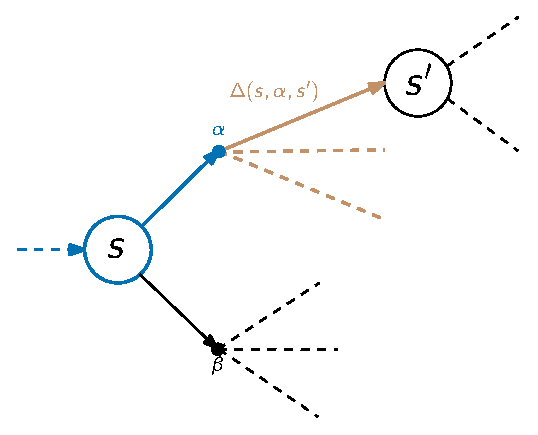
\includegraphics[width=0.45\linewidth]{resources/MDP-choice}
%   \end{figure}
%   \vspace{-0.05\linewidth}
%   \begin{itemize}
%     \item \textbf{\color{fibeamer@orange}Non-déterminisme} : en entrant dans un état $\color{fibeamer@blue}s$, une action $\color{fibeamer@blue}\alpha \in A(s)$ doit être choisie.
%     \item \textbf{\color{fibeamer@orange}Stochastique} : lorsqu'une action $\color{fibeamer@blue}\alpha \in A(s)$ est choisie, l'état suivant $\color{fibeamer@blue}s'$ est déterminé par la distribution de probabilité $\color{fibeamer@blue}\Delta(s, \alpha, \cdot)$ associée avec l'état courant $\color{fibeamer@blue}s$ et l'action $\color{fibeamer@blue}\alpha$ choisie.
%   \end{itemize}
% \end{frame}

\begin{frame}{Processus décisionnel de Markov (MDP)}{Exemple}\footnotesize
  \begin{figure}
    \centering
    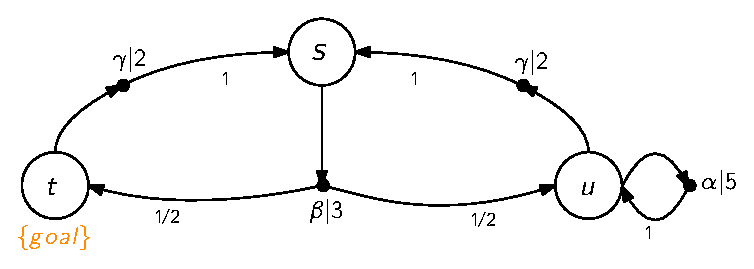
\includegraphics[width=0.65\linewidth]{resources/simple-mdp}
  \end{figure}
  \begin{columns}
    \begin{column}{0.4\linewidth}
      \begin{itemize}
        \item $S = \{s, t, u\}$
        \item $A = \{\alpha, \beta, \gamma\}$
        \item $L(t) = {\color{DarkOrange}\{goal\}}$
      \end{itemize}
    \end{column}
    \begin{column}{0.6\linewidth}
      \begin{itemize}
        \item $A(s) = \{\beta\}$,
        $A(t) = \{\gamma\}$,
        $A(u) = \{\alpha, \beta\}$
        \item $w(\alpha) = 5$, $w(\beta) = 3$, $w(\gamma) = 2$
        \item $\Delta(s_0, \beta, s_1) = \Delta(s_0, \beta, s_2) = \frac{1}{2}$
      \end{itemize}
    \end{column}
  \end{columns}
  \vspace{.02\linewidth} \textbf{\color{orange}Chemin :}
  \begin{overprint}
  \only<1>{
   $\color{fibeamer@blue}
     \pi = s_0 \xrightarrow{\alpha_1} s_1 \xrightarrow{\alpha_2} s_2 \xrightarrow{\alpha_3} \dots
   $
   où $\color{fibeamer@blue}\Delta(s_i, \alpha_{i+1}, s_{i+1}) > 0$, $\forall i \in \mathbb{N}$
  }\only<2>{
    $
      \pi = s \xrightarrow{\beta} t \xrightarrow{\gamma} s \xrightarrow{\beta}(u\xrightarrow{\alpha})^\omega \in Paths(s)
    $
    }
  \end{overprint}
\end{frame}

% \subsection{Chemins}
%
% \begin{frame}{Chemins}
%   Un \textit{\color{fibeamer@orange}chemin} dans un MDP $\mathcal{M} = (S, A, \Delta, w, AP, L)$ commençant en l'état $s \in S$ est une séquence infinie d'états et d'actions
%   \[\color{fibeamer@blue}
%     \pi = s_0 \xrightarrow{\alpha_1} s_1 \xrightarrow{\alpha_2} s_2 \xrightarrow{\alpha_3} \dots
%   \]
%   où $\color{fibeamer@blue}\Delta(s_i, \alpha_{i+1}, s_{i+1}) > 0$ avec $\alpha_{i+1} \in A(s_i)$ pour tout $i \in \mathbb{N}$.\\
%   \begin{itemize}
%     \item L'ensemble des chemins commençant en $s$ est dénoté par $\color{fibeamer@blue}Paths(s)$.
%   \end{itemize}
% \end{frame}
%
% \begin{frame}{Chemins}{Exemple}
%     \only<1-2>{  \begin{figure}
%         \centering
%         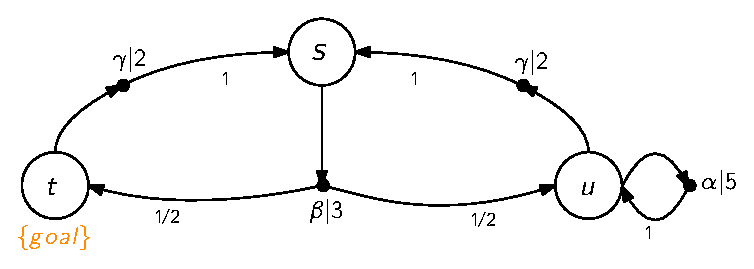
\includegraphics[width=0.85\linewidth]{resources/simple-mdp}
%       \end{figure}
%       }
%     \only<3>{ \begin{figure}
%         \centering
%         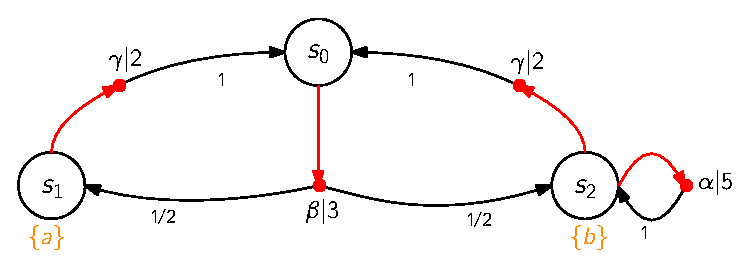
\includegraphics[width=0.85\linewidth]{resources/non-determ}
%       \end{figure}
%     }
%     \[
%       \pi = s_0 \xrightarrow{\beta} s_1 \xrightarrow{\gamma} s_0 \xrightarrow{\beta}(s_2\xrightarrow{\alpha})^\omega \in Paths(s_0)
%     \]
%     \vspace{-.07\linewidth}
%     \begin{itemize}
%       \item<2->[$\rightarrow$] \alert{Quelle est la probabilité de ce chemin ?}
%       \item<3>[$\rightarrow$] \alert{Non-déterminisme} $\color{fibeamer@blue}\implies$ on ne peut répondre à cette question sans aborder la notion de \textbf{\color{fibeamer@orange}stratégie}
%     \end{itemize}
% \end{frame}

\subsection{Stratégies}
\begin{frame}{Stratégies}\small
Une \textit{\color{fibeamer@orange}stratégie} $\color{fibeamer@blue} \sigma$ {\color{fibeamer@orange}choisit} à chaque étape une {\color{fibeamer@orange}action activée $\color{fibeamer@blue}\alpha \in A(s)$ de l'état courant $\color{fibeamer@blue}s$}
\begin{itemize}
  \item[$\rightarrow$] résout le non-déterminisme
  \item[$\rightarrow$] une stratégie peut utiliser...
  \begin{itemize}
    \item de la \textbf{\textit{\color{fibeamer@orange} mémoire}} (finie) : choisit les actions en fonction d'une quantité d'informations finie récoltée dans le passé
    \item de l'\textbf{\textit{\color{fibeamer@orange} aléatoire}} : choisit l'action selon une distribution de probabilité sur $\color{fibeamer@blue}A(s)$
  \end{itemize}
  \item[$\rightarrow$] les stratégies les plus simples sont les stratégies \textit{pures} (i.e., sans aléatoire) et sans mémoire $\leadsto$
  $
    \color{fibeamer@blue} \sigma: S \rightarrow A
  $
%   \item[$\rightarrow$] $\pi = s_0 \xrightarrow{\alpha_1} s_1 \xrightarrow{\alpha_2} s_2 \xrightarrow{\alpha_3} \dots$ est un $\color{fibeamer@blue}\sigma$-chemin ssi pour tout $i \in \mathbb{N}_0$, $\alpha_i$ est une action choisie par $\color{fibeamer@blue}\sigma$
%   \begin{itemize}
%     \item[$\leadsto$] l'ensemble de ces $\sigma$-chemins commençant en l'état $s \in S$ est dénoté par $\color{fibeamer@blue}Paths^\sigma(s)$
%   \end{itemize}
\end{itemize}
\end{frame}

% \begin{frame}{Stratégies}{Exemple}\small
% \begin{figure}
%         \centering
%         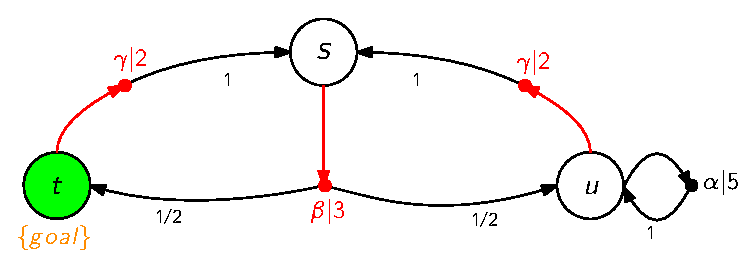
\includegraphics[width=0.8\linewidth]{resources/strat-ex}
%       \end{figure}
%   \begin{itemize}
%     \item $\color{red}\sigma$ est une stratégie pure et sans mémoire
%     \item ${\color{red}\sigma}(s_0) = \beta$,
%     ${\color{red}\sigma}(s_1) = \gamma$,
%     ${\color{red}\sigma}(s_2) = \alpha$
%     \item $\pi = s_0 \xrightarrow{\beta} s_1 \xrightarrow{\gamma} s_0 \xrightarrow{\beta}(s_2\xrightarrow{\alpha})^\omega \in {\color{red}Paths^\sigma(s_0)}$
%   \end{itemize}
% \end{frame}

\begin{frame}{Chaîne de Markov induite par stratégie}\small
Une fois que la \textbf{\color{fibeamer@orange}stratégie contrôle les décisions du MDP}, ce dernier a un \textbf{\color{fibeamer@orange}comportement purement stochastique}
\begin{itemize}
  \item[$\rightarrow$] Une chaîne de Markov est induite par la stratégie
  % \item Un espace probabiliste équipé de la mesure de probabilité $\color{fibeamer@blue}\mathbb{P}^\sigma_s$
  %  est associée avec toute chaîne de Markov, permettant de \textbf{\color{fibeamer@orange} mesurer la probabilité} des \textbf{\color{fibeamer@orange}évènement} $\color{fibeamer@blue}E \subseteq Paths^\sigma(s)$ avec $\color{fibeamer@blue}\mathbb{P}^\sigma_s(E) \in [0, 1] \cap \mathbb{Q}$
  \item On peut mesurer la probabilité des \textbf{\color{fibeamer@orange}évènements} $\color{fibeamer@blue}E \subseteq Paths(s)$ dans la chaîne de Markov induite par toute stratégie $\color{red}\sigma$ {\color{fibeamer@blue}$\leadsto$} $\mathbb{P}_s^{{\color{red}\sigma}}({\color{fibeamer@blue}E})$

  %\item \textit{\color{fibeamer@blue}Exemples}:
    \begin{itemize}
      \item ${\color{fibeamer@blue}\Diamond T}
      %= \{\pi = s_0s_1s_2 \dots \; | \; \exists n \in \mathbb{N}, \, s_n \in T \}
      = \{\pi = s_0s_1s_2\dots \in Paths(\mathcal{M}) \; | \; \exists n \in \mathbb{N}, \; s_n \in T \}$ \item[$\leadsto$] \textbf{\color{fibeamer@orange}atteindre} $\color{fibeamer@blue} T$, où $T \subseteq S$ est un sous-ensemble d'\textbf{\color{fibeamer@orange}états cibles}% $\leadsto \mathbb{P}_{s_0}^{{\color{red}\sigma}}(\Diamond \{s_2\}) = 1$
      %\item \textbf{\color{fibeamer@orange} atteindre} $\color{fibeamer@blue}\{s_2\}$ \textbf{\color{fibeamer@orange}en visitant une fois} $\color{fibeamer@blue}s_1$ $\leadsto \mathbb{P}_{s_0}^{{\color{red}\sigma}}(\{s_0s_1s_0s_2^\omega\}) = \frac{1}{2} \cdot 1 \cdot \frac{1}{2} \cdot 1^\omega = \frac{1}{4}$
      \item $? \exists \alert{\sigma}$, $\; \mathbb{P}^{\alert{\sigma}}_{s}(\Diamond {\color{green}\{t\}}) = 1$
      %\item[$\rightarrow$] oui :
    \end{itemize}
\begin{columns}
  \begin{column}{0.5\linewidth}
    \begin{figure}
            \centering
            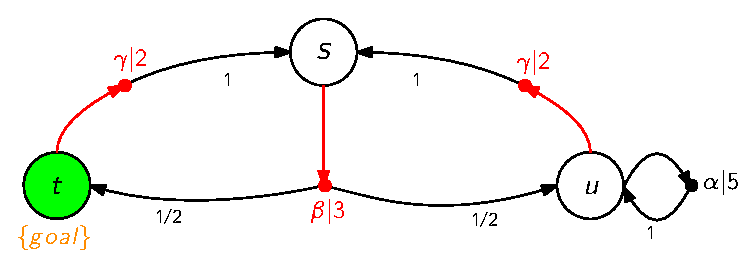
\includegraphics[width=\linewidth]{resources/strat-ex}
    \end{figure}
  \end{column}
  \begin{column}{0.5\linewidth}
    \begin{figure}
            \centering
            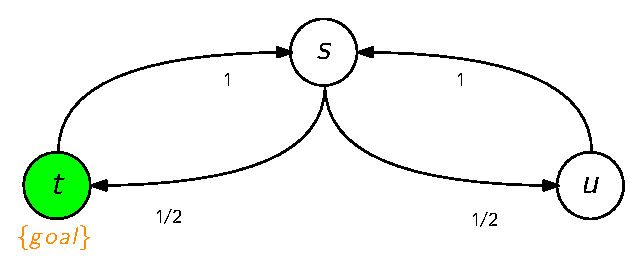
\includegraphics[width=0.85\linewidth]{resources/inducted-markov1}
    \end{figure}
  \end{column}
\end{columns}
\end{itemize}
  % \begin{itemize}
  %   \item[$\leadsto$] $\pi = s_0 {\color{red}\xrightarrow{\beta}} s_1 {\color{red}\xrightarrow{\gamma}} s_0 {\color{red}\xrightarrow{\beta}}(s_2{\color{red}\xrightarrow{\alpha}})^\omega\in Paths^{\color{red}\sigma}(s_0)$
  %   \item[$\leadsto$] $\mathbb{P}_{s_0}^{{\color{red}\sigma}}(\{s_0s_1s_0s_2^\omega\}) = \frac{1}{2} \cdot 1 \cdot \frac{1}{2} \cdot 1^\omega = \frac{1}{4}$
  % \end{itemize}
\end{frame}

% \begin{frame}{PRCTL}{Quelques exemples}
%     \begin{figure}
%       \centering
%       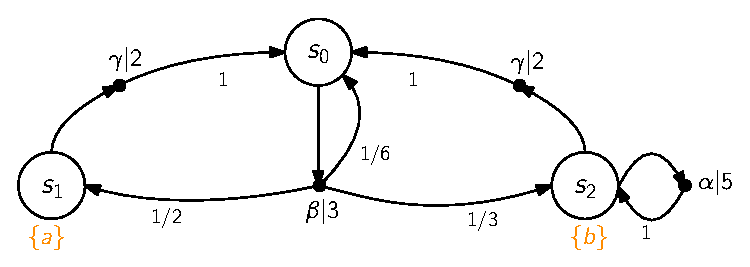
\includegraphics[width=0.7\linewidth]{resources/MDP2}
%     \end{figure}
%     \begin{itemize}
%       \item[-] \textbf{\color{orange}Accessibilité répétée}: ``visiter $\color{DarkOrange}a$ infiniment souvent avec une \textit{probabilité maximale} supérieure ou égale à $\frac{1}{2}$''
%       \item[-] \textbf{\color{orange}Persistance} :  ``Visiter $\color{DarkOrange}b$ à chaque étape, avec une \textit{probabilité maximale} de $1$''
%       \item[-] \textbf{\color{orange}Accessibilité limitée} : ``accéder à $\color{DarkOrange}a$ avec un coût inférieur à 8 tout en évitant $\color{DarkOrange}b$ avec une \textit{probabilité maximale} supérieure ou égale à $\frac{1}{5}$''
%     \end{itemize}
% \end{frame}

\section{Synthèse}

\subsection{Introduction}


% \begin{frame}{Plus court chemin stochastique}\footnotesize
% \vspace{-.05\linewidth}
%   \begin{itemize}
%     \item Les problèmes de décision multi-objectifs présentés concernent le problème de \textit{\color{orange}plus court chemin stochastique}
%     %\item \`A une dimension $\leadsto$ projet de master 1
%     \item La fonction utilisée pour calculer le coût des chemins est la \textbf{\textit{\color{fibeamer@orange}somme tronquée}}:
%     \begin{itemize}
%       \footnotesize
%       %\item soit $\color{fibeamer@blue}\mathcal{M}$ un MDP avec un espace d'états $\color{fibeamer@blue}S$,
%       %un espace d'action $\color{fibeamer@blue}A$
%       %et une fonction de pondération $\color{fibeamer@blue}w$
%       \item soit $\color{fibeamer@blue}T \subseteq S$ un {\color{fibeamer@blue}ensemble d'états cibles}, et $\pi = s_0\xrightarrow{\alpha_1}s_1\xrightarrow{\alpha_2}s_2\xrightarrow{\alpha_3}\dots \in Paths(\mathcal{M})$
%     \end{itemize}
%   \end{itemize}
%       \[
%         {\color{fibeamer@blue}\TS^T(\pi)}=\begin{cases}
%           \sum_{i=1}^{n} w(\alpha_i) & \text{si } s_n \text{ est la première visite de }T,\\
%           + \infty & \text{si } T \text{ n'est jamais atteint dans } \pi
%         \end{cases}
%       \]
%       \vspace{-.02\linewidth}
%     \begin{columns}
%       \begin{column}{0.5\linewidth}
%     \begin{figure}
%             \centering
%             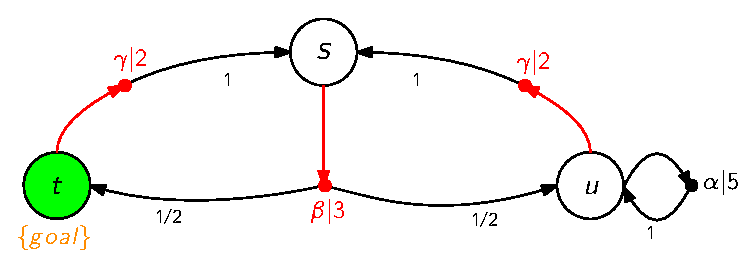
\includegraphics[width=\linewidth]{resources/strat-ex}
%     \end{figure}
%       \end{column}
%       \begin{column}{0.5\linewidth}
%     \begin{itemize}
%       \item[$\leadsto$] $\pi = (s_0 {\color{red}\xrightarrow{\beta}} s_2 {\color{red}\xrightarrow{\gamma}} s_0 {\color{red}\xrightarrow{\beta}}s_1{\color{red}\xrightarrow{\gamma}})^\omega$
%       \item $\TS^{\{s_1\}}(\pi) = w(\alert{\beta}) + w(\alert{\gamma}) + w(\alert{\beta}) = \alert{3} + \alert{2} + \alert{3} = 8$
%       \end{itemize}
%       \end{column}
%     \end{columns}
% \end{frame}

\begin{frame}{Problèmes de décisions}\footnotesize
  Existe-t-il une stratégie $\color{fibeamer@blue}\sigma$ qui satisfait ...\\[0.3em]
  \textbf{\itshape \color{fibeamer@orange}Problèmes mono-objectifs}
  \begin{itemize}
    \item \textbf{\color{fibeamer@blue}SR} : une haute probabilité d'accessibilité stochastique
    \item \textbf{\color{fibeamer@blue}SSP-E} : une bonne espérance du coût pour atteindre la cible
    \item \textbf{\color{fibeamer@blue}SSP-P} : une accessibilité à la cible avec un coût limité sous une haute probabilité
    \item \textbf{\color{fibeamer@blue}SP-G} : une garantie d'une borne en terme de coût pour atteindre la cible
  \end{itemize}
  \textbf{\itshape \color{fibeamer@orange}Problèmes multi-objectifs}
  \begin{itemize}
    \item \textbf{\color{fibeamer@blue}SSP-WE} : une bonne espérance du coût pour atteindre la cible sous une garantie de pire cas
    \item \textbf{\color{fibeamer@blue}MOSR} : plusieurs problèmes \textbf{\color{fibeamer@blue}SR}
    \textit{\color{fibeamer@orange}simultanément}
    \item \textbf{\color{fibeamer@blue}SSP-PQ} : plusieurs problèmes \textbf{\color{fibeamer@blue}SSP-P}
    \textit{\color{fibeamer@orange}simultanément}
  \end{itemize}
\end{frame}

\begin{frame}{Problèmes de décisions}\footnotesize
  \addtocounter{framenumber}{-1}
  Existe-t-il une stratégie $\color{fibeamer@blue}\sigma$ qui satisfait ...\\[0.3em]
  \textbf{\itshape \color{fibeamer@orange}Problèmes mono-objectifs}
  \begin{itemize}
    \color{lightgray}
    \item[\color{lightgray}{\textbullet}] \textbf{SR} : une haute probabilité d'accessibilité stochastique
    \item {\color{black}\textbf{\color{fibeamer@blue}SSP-E} : une bonne espérance du coût pour atteindre la cible}
    \item[\color{lightgray}{\textbullet}] \textbf{SSP-P} : une accessibilité à la cible avec un coût limité sous une haute probabilité
    \item[\color{lightgray}{\textbullet}] \textbf{SP-G} : une garantie d'une borne en terme de coût pour atteindre la cible
  \end{itemize}
  \textbf{\itshape \color{fibeamer@orange}Problèmes multi-objectifs}
  \begin{itemize}
  \color{lightgray}
    \item {\color{black} \textbf{\color{fibeamer@blue}SSP-WE} : une bonne espérance du coût pour atteindre la cible sous une garantie de pire cas}
    \item[\color{lightgray}{\textbullet}] \textbf{MOSR} : plusieurs problèmes \textbf{SR}
    \textit{simultanément}
    \item[\color{lightgray}{\textbullet}] \textbf{SSP-PQ} : plusieurs problèmes \textbf{SSP-P}
    \textit{simultanément}
  \end{itemize}
\end{frame}

% \begin{frame}\footnotesize
%   \begin{block}{\small Le problème d'accessibilité stochastique (SR)}
%     Soit $\color{fibeamer@blue}\mathcal{M}$ un MDP dont l'espace d'état est $S$, $\color{fibeamer@blue}s \in S$ un état de $\mathcal{M}$, $\color{fibeamer@blue}T \subseteq S$ {\color{fibeamer@orange}un ensemble d'états cibles}, et un {\color{fibeamer@orange}seuil de probabilité}  $\color{fibeamer@blue}\alpha \in [0, 1]\cap\mathbb{Q}$%, et $\color{fibeamer@blue}\ell \in \mathbb{N}_0$
%     \begin{itemize}
%     \item {\color{fibeamer@orange}\textbf{\'Evènement} : $\Diamond T$} $\leadsto$ atteindre $T$
%     \vspace{-.02\linewidth}
%     \[\color{fibeamer@blue}? \exists \sigma, \, \mathbb{P}^\sigma_s(\Diamond T) \geq \alpha\]
%     \vspace{-.07\linewidth}
%       \item[$\rightarrow$] \textit{existe-t-il une stratégie permettant d'atteindre $T$ depuis $s$ avec une probabilité supérieure à $\alpha$ ?}
%       \item peut être décidé en \textbf{\color{orange}temps polynomial en la taille de $\mathcal{M}$} par \textbf{\color{orange}programmation linéaire}
%       \item
%       %Si une stratégie satisfaisant le problème existe,
%       $\color{fibeamer@orange}\exists \sigma \implies$\textbf{\color{fibeamer@orange}la stratégie optimale} est construite en temps polynomial en la taille de $\mathcal{M}$ et est \textbf{\color{fibeamer@orange}pure et sans mémoire}
%     \end{itemize}
%   \end{block}
%   %  \vspace{-.02\linewidth}
%   \begin{figure}
%     \centering
%     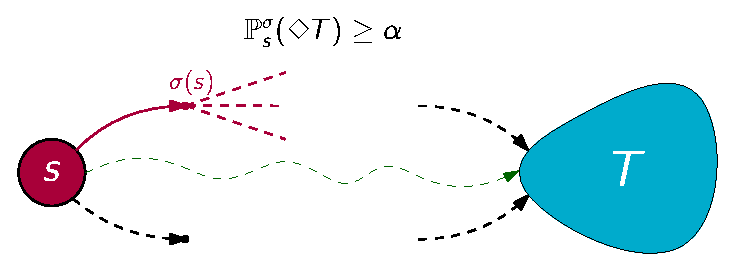
\includegraphics[width=0.55\linewidth]{resources/SR}
%   \end{figure}
% \end{frame}
%
% \begin{frame}\footnotesize
%   \begin{block}{\small Plus court chemin stochastique : coût attendu jusqu'à la cible (SSP-E)}
%     Soit $\color{fibeamer@blue}\mathcal{M}$ un MDP dont l'espace d'état est $S$, $\color{fibeamer@blue}s \in S$ un état de $\mathcal{M}$, $\color{fibeamer@blue}T \subseteq S$ {\color{fibeamer@orange}un ensemble d'états cibles}, et un {\color{fibeamer@orange}seuil de coût}  $\ell \in \mathbb{N}_0$%, et $\color{fibeamer@blue}\ell \in \mathbb{N}_0$
%     %\vspace{-.02\linewidth}
%     \[\color{fibeamer@blue}? \exists \sigma, \, \mathbb{E}^\sigma_s(\TS^T) \leq \ell\]
%     \vspace{-.05\linewidth}
%     \begin{itemize}
%       \item[$\rightarrow$] \textit{existe-t-il une stratégie permettant d'atteindre $T$ depuis $s$ avec un coût moyen attendu inférieur à $\ell$ ?}
%       \item peut être décidé en \textbf{\color{orange}temps polynomial en la taille de $\mathcal{M}$} par \textbf{\color{orange}programmation linéaire}
%       \item $\color{fibeamer@orange}\exists \sigma \implies$ \textbf{\color{fibeamer@orange}la stratégie optimale} peut être construite en temps polynomial en la taille de $\mathcal{M}$ et est \textbf{\color{fibeamer@orange}pure et sans mémoire}
%     \end{itemize}
%   \end{block}
%   %  \vspace{-.02\linewidth}
%   \begin{figure}
%     \centering
%     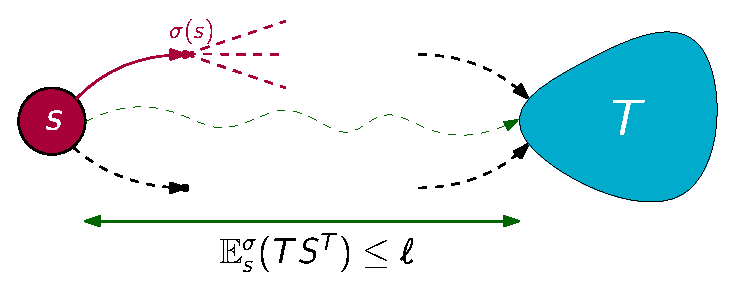
\includegraphics[width=0.6\linewidth]{resources/SSPE}
%   \end{figure}
% \end{frame}
%
% \begin{frame}\footnotesize
%   \begin{block}{\small Problème du plus court chemin stochastique percentile (SSP-P)}
%     Soit $\color{fibeamer@blue}\mathcal{M}$ un MDP dont l'espace d'état est $S$, $\color{fibeamer@blue}s \in S$ un état de $\mathcal{M}$, $\color{fibeamer@blue}T \subseteq S$ {\color{fibeamer@orange}un ensemble d'états cibles}, un {\color{fibeamer@orange}seuil de coût} $\ell \in \mathbb{N}_0$, et un {\color{fibeamer@orange}seuil de probabilité}  $\color{fibeamer@blue}\alpha \in [0, 1]\cap\mathbb{Q}$
%     %, et $\color{fibeamer@blue}\ell \in \mathbb{N}_0$
%     \begin{itemize}
%     \item {\color{fibeamer@orange}\textbf{\'Evènement} : $\Diamond_{\leq \ell} \, T$}$\leadsto$ %\{\pi \in Paths(s)\; | \; \TS^T(\pi) \leq \ell \}$
%     atteindre $T$ avec un coût inférieur à $\ell$
%     \vspace{-.01\linewidth}
%     \[\color{fibeamer@blue}? \exists \sigma, \, \mathbb{P}^\sigma_s(\Diamond_{\leq \ell} \, T) \geq \alpha\]
%     \vspace{-.07\linewidth}
%       \item[$\rightarrow$] \textit{existe-t-il une stratégie permettant d'atteindre $T$ depuis $s$ avec un coût inférieur à $\ell$ et avec une probabilité supérieure à $\alpha$ ?}
%       \item peut être décidé en \textbf{\color{orange}temps polynomial en la taille de $\mathcal{M}$}, mais en
%       \textbf{\color{orange}temps \textit{pseudo-polynomial} en la taille de la taille de l'entrée $\ell$}
%       \item
%       %Si une stratégie satisfaisant le problème existe,
%       $\color{fibeamer@orange}\exists \sigma \implies$\textbf{\color{fibeamer@orange}la stratégie optimale} est construite en temps pseudo-polynomial et est \textbf{\color{fibeamer@orange}pure et à mémoire pseudo-polynomiale}
%     \end{itemize}
%   \end{block}
%   \vspace{-.02\linewidth}
%   \begin{figure}
%     \centering
%     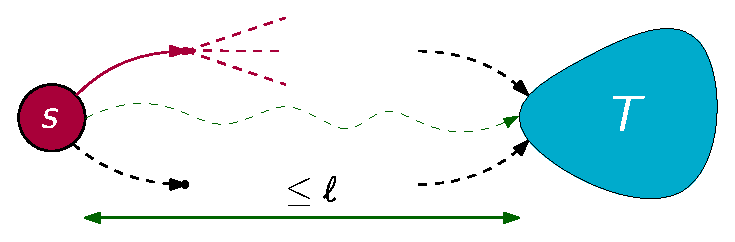
\includegraphics[width=0.55\linewidth]{resources/SSPP}
%   \end{figure}
% \end{frame}

\begin{frame}{Problème multi-objectif : exemple}{Communication entre noeuds dans un réseau de capteurs}\footnotesize
\begin{columns}
\begin{column}{0.4\linewidth}
  \begin{center}
    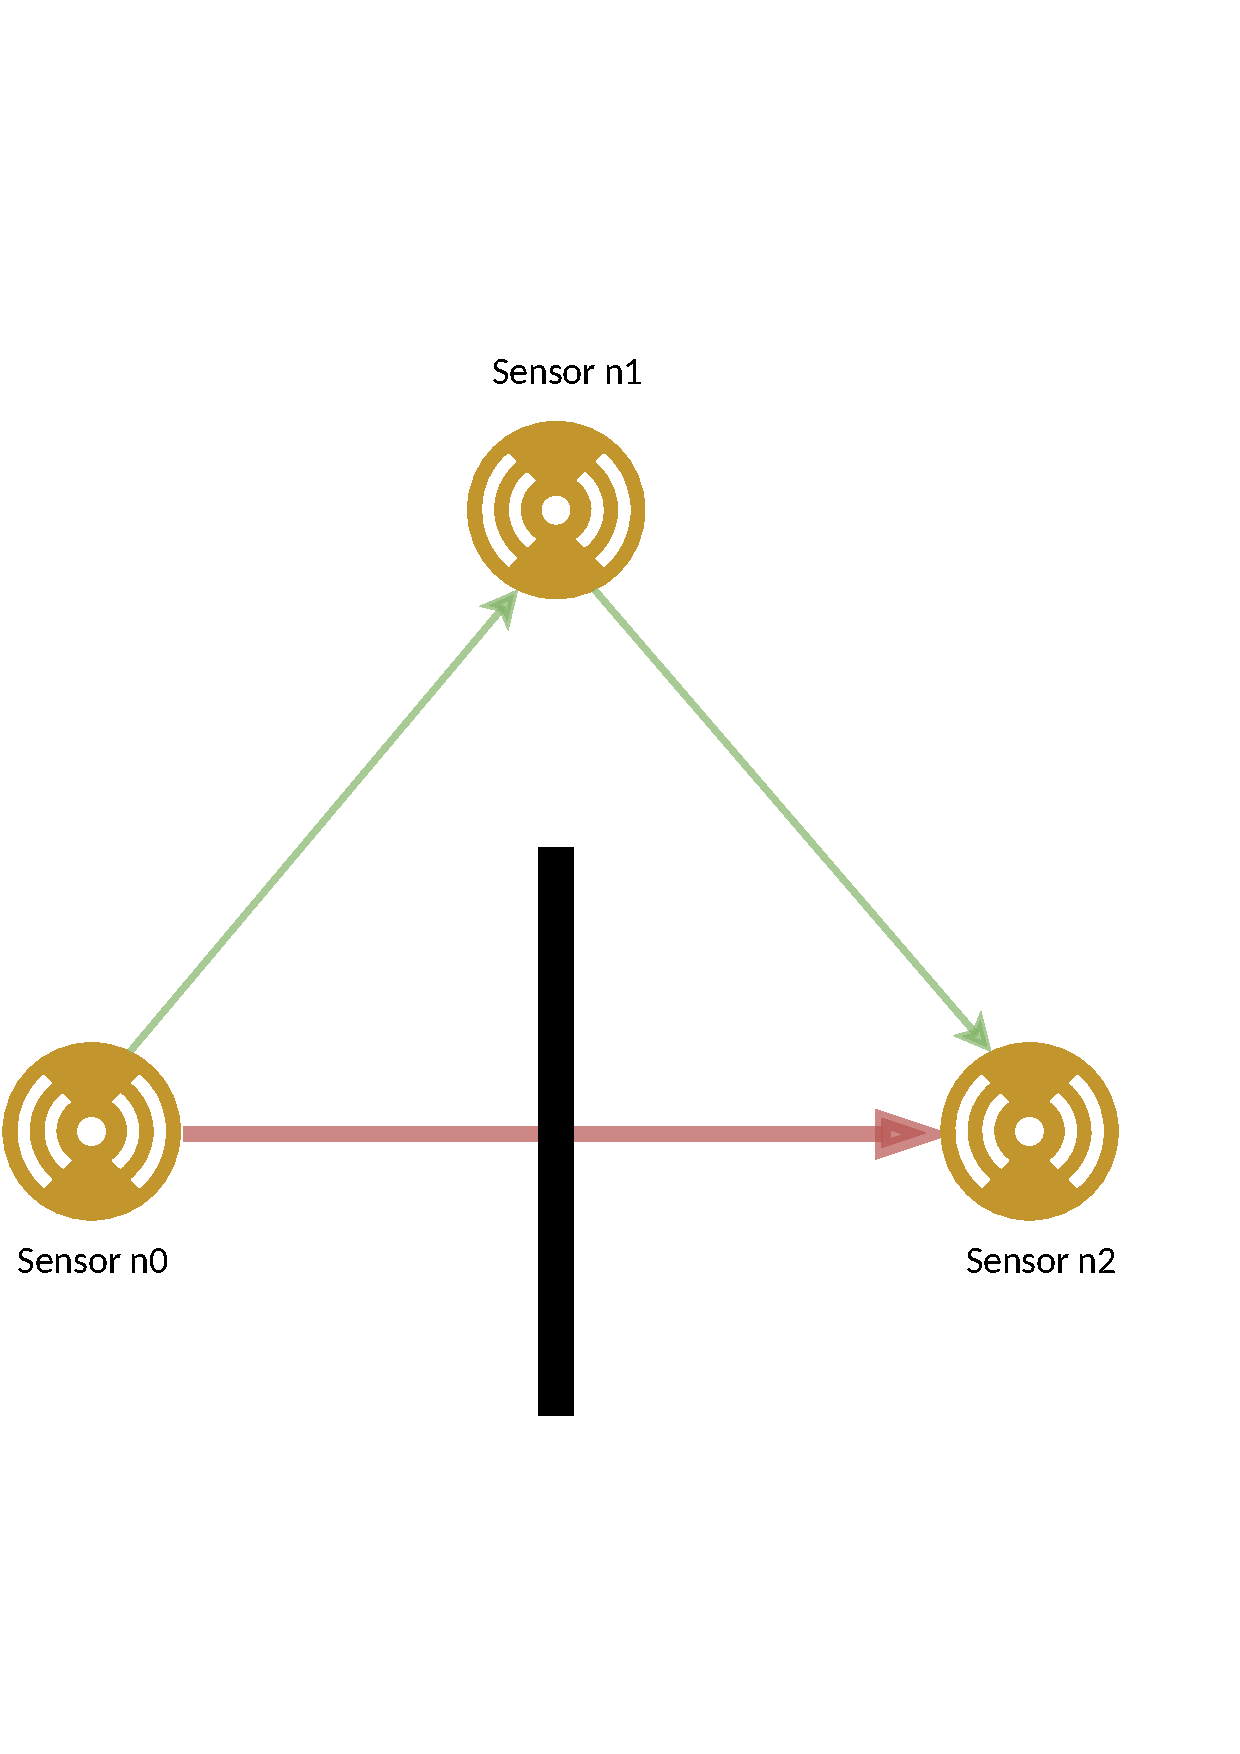
\includegraphics[width=\linewidth]{resources/example2.pdf}
  \end{center}
\end{column}
\begin{column}{0.6\linewidth}
    \vspace{-.03\linewidth}
    \begin{itemize}
      \item Un obstacle sépare $n_0$ et $n_2$
      \item Communication directe $n_0 \rightarrow n_2$
      \vspace{-.03\linewidth}
      \begin{itemize}
      \footnotesize
        \item[$\leadsto$] plus rapide que de passer par un noeud intermédiaire
        %\item[$\leadsto$] nécessite plus d'énergie
        \item[$\leadsto$] risque de corruption des paquets envoyés (bruit)
      \end{itemize}
      \vspace{-.04\linewidth}
      \item Communication indirecte : $n_0 \rightarrow n_1 \rightarrow n_2$
      \vspace{-.1\linewidth}
      \begin{itemize}
        \footnotesize
        \item[$\leadsto$] plus lent ($n_1$ doit attendre la confirmation de réception du paquet par $n_2$ et $n_0$ doit attendre la confirmation de $n_1$)
        %\item[$\leadsto$] consommation d'énergie normale
        \item[$\leadsto$] risque de corruption de paquet négligeable
      \end{itemize}
    \end{itemize}
\end{column}
\end{columns}
\end{frame}

\begin{frame}{Problème multi-objectif : exemple}{Communication entre noeuds dans un réseau de capteurs}
  \begin{center}
    \only<1>{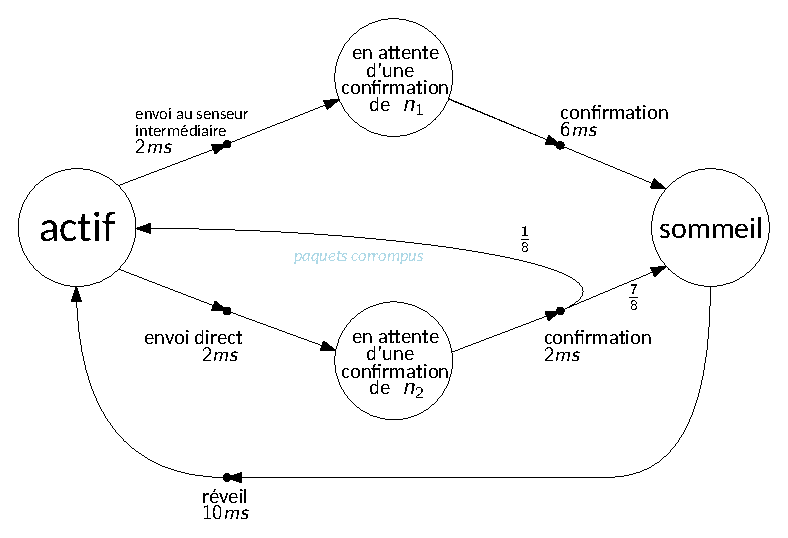
\includegraphics[width=0.7\linewidth]{resources/main-mdp}}
    \only<2>{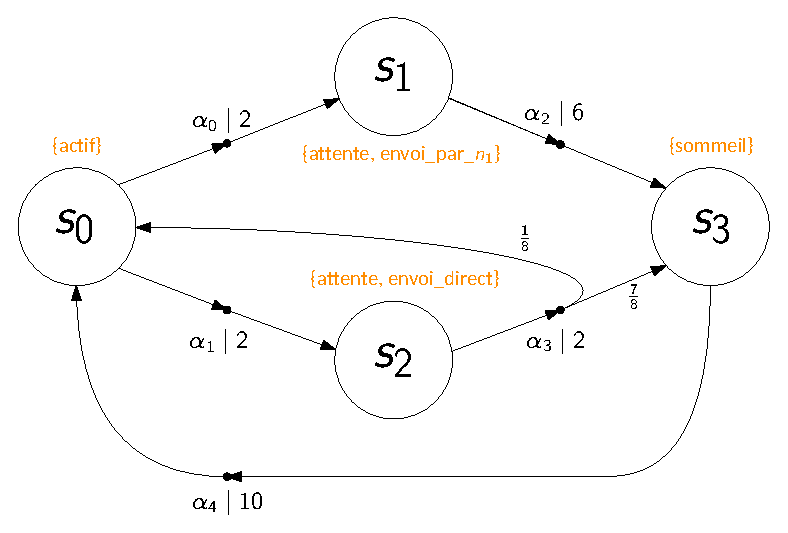
\includegraphics[width=0.7\linewidth]{resources/main-mdp3}}
  \end{center}
\end{frame}

\begin{frame}{Plus court chemin stochastique}{Somme tronquée}
%\vspace{-.05\linewidth}
  \begin{itemize}
    \item Les problèmes de décision présentés concernent le problème de \textit{\color{orange}plus court chemin stochastique}
    %\item \`A une dimension $\leadsto$ projet de master 1
    \item Calculer le coût des chemins $\color{fibeamer@blue}\leadsto$ \textbf{\textit{\color{fibeamer@orange}somme tronquée}}:\\
    \begin{itemize}
      %\item soit $\color{fibeamer@blue}\mathcal{M}$ un MDP avec un espace d'états $\color{fibeamer@blue}S$,
      %un espace d'action $\color{fibeamer@blue}A$
      %et une fonction de pondération $\color{fibeamer@blue}w$
      \item soit $\color{fibeamer@blue}T \subseteq S$ un {\color{fibeamer@blue}ensemble d'états cibles}, et $\pi = s_0\xrightarrow{\alpha_1}s_1\xrightarrow{\alpha_2}s_2\xrightarrow{\alpha_3}\dots \in Paths(\mathcal{M})$
    \end{itemize}
  \end{itemize}
      \[
        {\color{fibeamer@blue}\TS^T(\pi)}=\begin{cases}
          \sum_{i=1}^{n} w(\alpha_i) & \text{si } s_n \text{ est la première visite de }T,\\
          + \infty & \text{si } T \text{ n'est jamais atteint dans } \pi
        \end{cases}
      \]
  %   \vspace{-.02\linewidth}
  % \begin{columns}
  %   \begin{column}{0.5\linewidth}
  % \begin{figure}
  %         \centering
  %         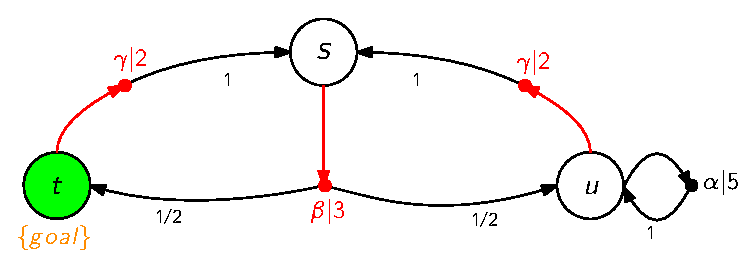
\includegraphics[width=\linewidth]{resources/strat-ex}
  % \end{figure}
  %   \end{column}
  %   \begin{column}{0.5\linewidth}
  % \begin{itemize}
  %   \item[$\leadsto$] $\pi = (s_0 {\color{red}\xrightarrow{\beta}} s_2 {\color{red}\xrightarrow{\gamma}} s_0 {\color{red}\xrightarrow{\beta}}s_1{\color{red}\xrightarrow{\gamma}})^\omega$
  %   \item $\TS^{\{s_1\}}(\pi) = w(\alert{\beta}) + w(\alert{\gamma}) + w(\alert{\beta}) = \alert{3} + \alert{2} + \alert{3} = 8$
  %   \end{itemize}
  %   \end{column}
  % \end{columns}
\end{frame}

\subsection{SSP-E}

\begin{frame}{Plus court chemin stochastique}{SSP-E : Bonne espérance de coût pour atteindre la cible}\small
\begin{itemize}
  \item $\mathbb{E}[X] = \sum_{i} x_i \cdot \mathbb{P}(X=x_i)$
  \begin{itemize}
    \item[$\leadsto$] moyenne pondérée par les probabilités
  \end{itemize}
  \item $\color{fibeamer@blue}\mathbb{E}^\sigma_s(\TS^T)$
  : coût moyen attendu pour atteindre $\color{fibeamer@blue}T$ depuis $\color{fibeamer@blue}s$
  \[ \color{fibeamer@blue}
    ? \exists \sigma,\; \mathbb{E}^\sigma_s(\TS^T) \leq \ell
  \]
  \item<2> Peut être résolu par \textbf{\color{fibeamer@orange}programmation linéaire} en temps \textbf{\color{fibeamer@orange}polynomial en la taille du modèle}
  \item<2> Requiert une stratégie \textbf{\color{fibeamer@orange}pure} et \textbf{\color{fibeamer@orange}sans mémoire}
\end{itemize}
\end{frame}

\begin{frame}{Plus court chemin stochastique}{SSP-E : Bonne espérance de coût pour atteindre la cible}
  \[ \color{fibeamer@blue}
    ? \exists \sigma,\; \mathbb{E}^\sigma_s(\TS^\text{ \color{DarkOrange} sommeil}) \leq 6
  \]
\begin{columns}
  \begin{column}{0.5\linewidth}
    \begin{overprint}
      \onslide<1>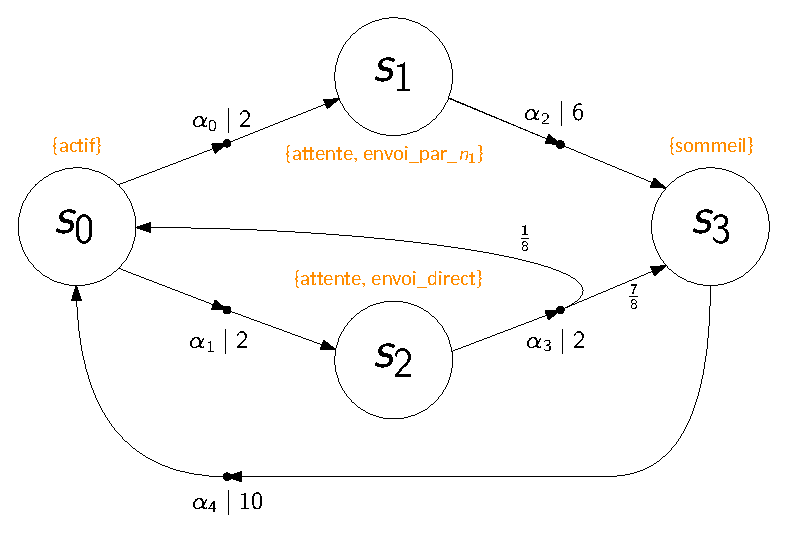
\includegraphics[width=\linewidth]{resources/main-mdp6}
      \onslide<2>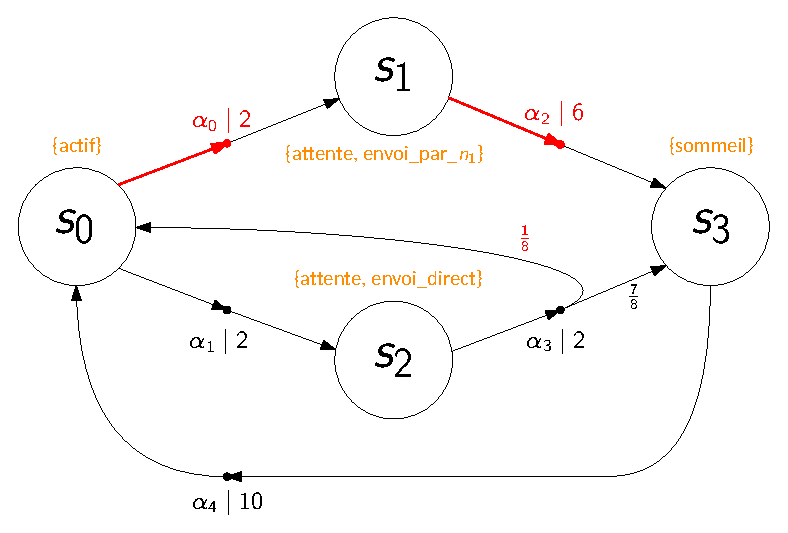
\includegraphics[width=\linewidth]{resources/SPG1}
      \onslide<3>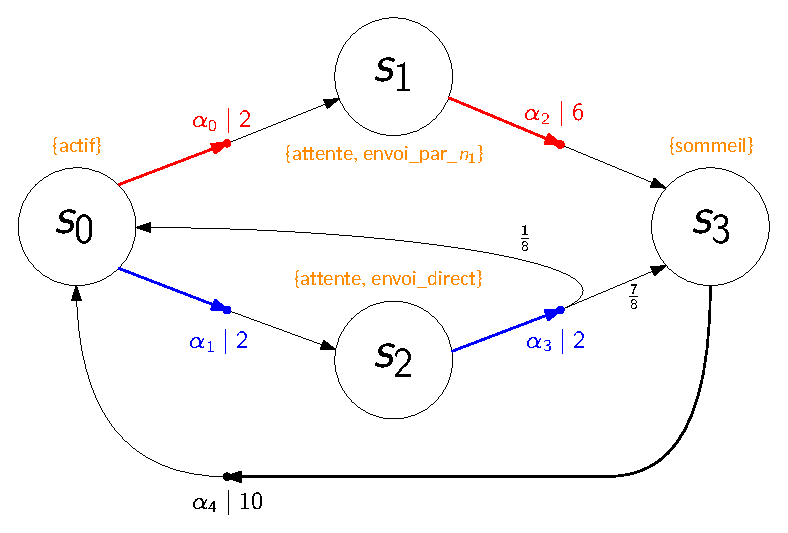
\includegraphics[width=\linewidth]{resources/SPG2}
      \onslide<4>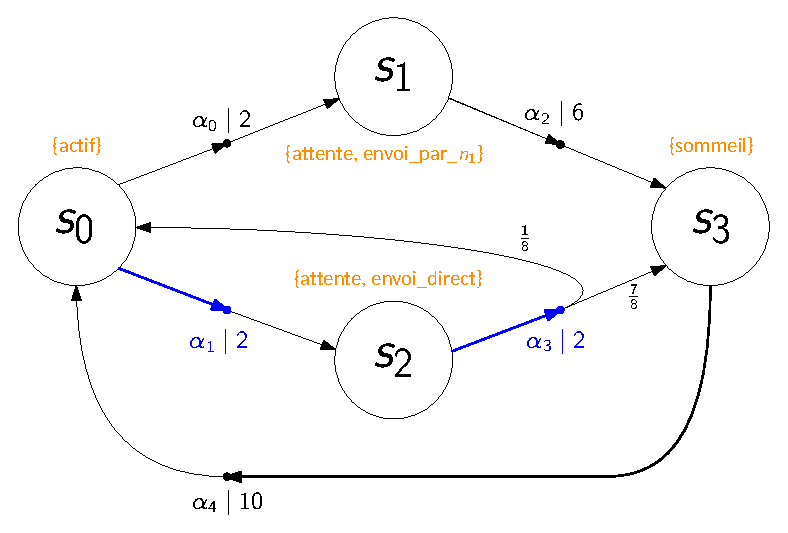
\includegraphics[width=\linewidth]{resources/SPG3}
    \end{overprint}
  \end{column}
  \begin{column}{0.5\linewidth}
    \begin{itemize}
      \item<2-> \only<2-3>{$\mathbb{E}^{{\color{red}\sigma}}_{s_0}(\TS^{\color{DarkOrange}\text{ sommeil}}) = 8$}
      \only<4>{ $\cancel{\mathbb{E}^{{\color{red}\sigma}}_{s_0}(\TS^{\color{DarkOrange}\text{ sommeil}}) = 8 {\color{red} > 6}}$}
      \item<3-> $\mathbb{E}^{{\color{blue}\sigma}}_{s_0}(\TS^{\color{DarkOrange}\text{ sommeil}}) = 4.57$ \only<4>{$\color{fibeamer@orange}\leq 6$}
    \end{itemize}
  \end{column}
\end{columns}
\end{frame}

% \subsection{SP-G}
%
% \begin{frame}{Plus court chemin : jeu}{Shortest path game $-$ SP-G}\small
%   \begin{itemize}
%     \item Supposons que l'on veuille {\color{fibeamer@blue}assurer} une \textbf{\color{orange}garantie} {\color{fibeamer@blue}d'atteindre} un ensemble d'états cibles $\color{fibeamer@blue}T$ avec un {\color{fibeamer@blue}coût inférieur} à un seuil $\color{fibeamer@blue}\ell$
%   \end{itemize}
%   \begin{columns}
%     \begin{column}{0.5\linewidth}
%         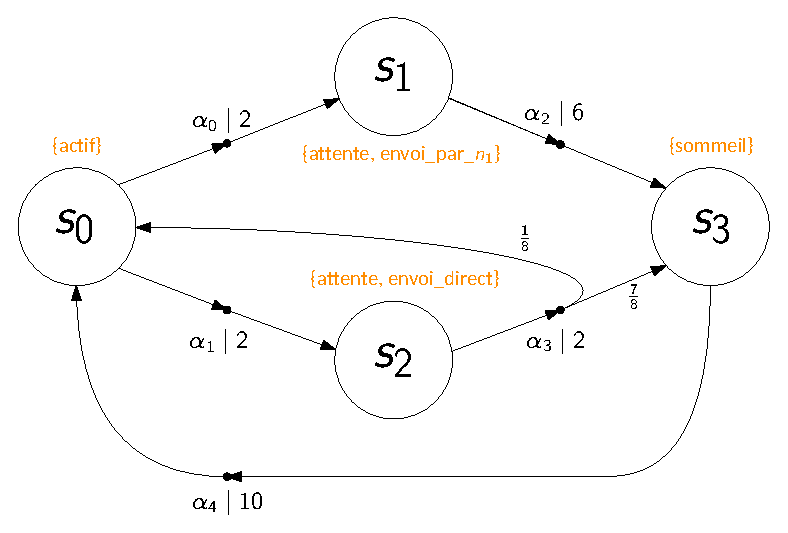
\includegraphics[width=\linewidth]{resources/main-mdp3}
%     \end{column}
%     \begin{column}{0.5\linewidth}\footnotesize
%       \begin{itemize}
%         \item[$\rightarrow$] Garantir un \textbf{\color{fibeamer@orange}duty cycle} de $12$ $ms$ ?
%         \item[$\rightarrow$] $? \exists \sigma, \, \forall \pi \in Paths^\sigma(s_0)$, $\TS^{\text{\color{DarkOrange} sommeil}}(\pi) \leq 12$
%       \end{itemize}
%     \end{column}
%   \end{columns}
% \end{frame}

% \begin{frame}{Plus court chemin : jeu}
%   \textbf{\color{fibeamer@blue}Idée : } considérer le MDP comme un jeu à deux joueurs et \textit{``oublier les probabilités''}
%     \begin{itemize}
%       \item \textbf{Joueur 1} : choisit l'action
%       \item \textbf{Joueur 2} : \textbf{\color{orange}adversaire $\rightarrow$} choisit le successeur $s'$ $\leadsto$ l'état qui mène au pire cas en terme de somme tronquée
%     \end{itemize}
%   \begin{columns}
%     \begin{column}{0.5\linewidth}
%       \begin{overprint}
%         \onslide<1>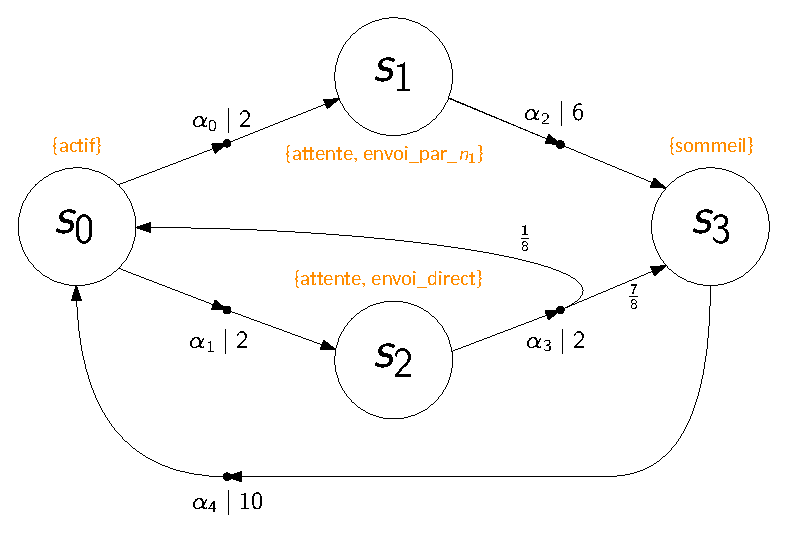
\includegraphics[width=\linewidth]{resources/main-mdp6}
%         \onslide<2>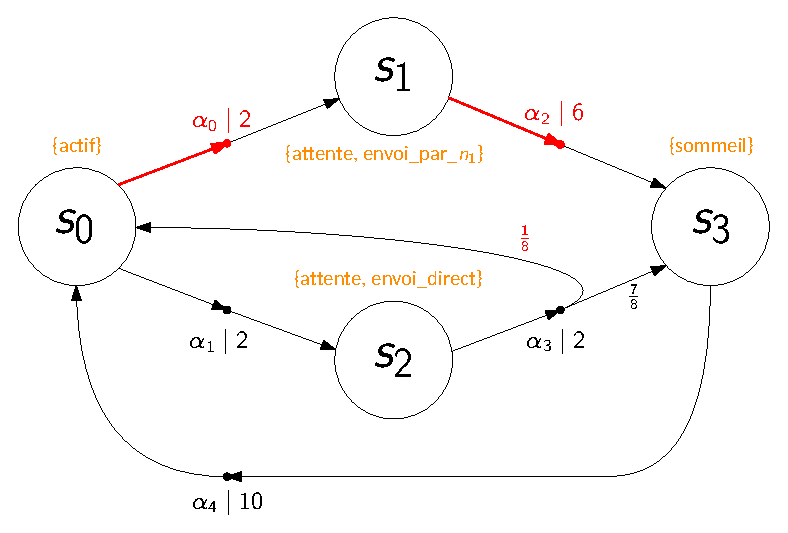
\includegraphics[width=\linewidth]{resources/SPG1}
%         \onslide<3>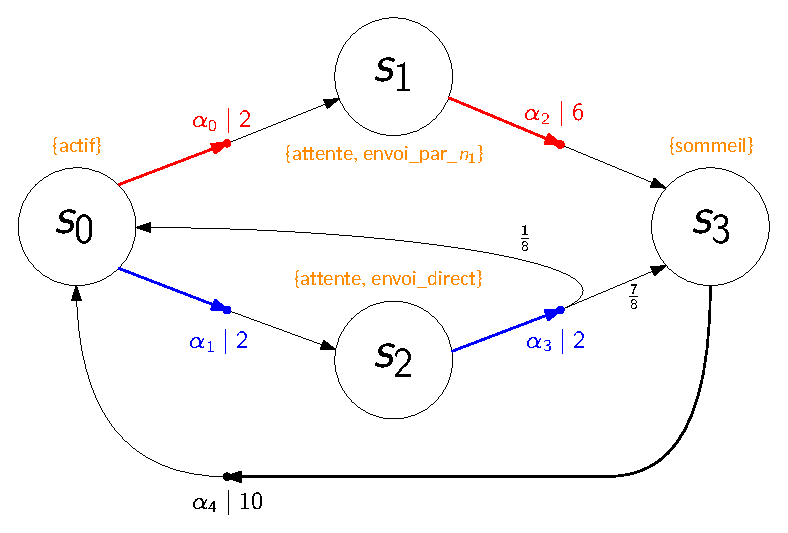
\includegraphics[width=\linewidth]{resources/SPG2}
%       \end{overprint}
%     \end{column}
%     \begin{column}{0.5\linewidth}\footnotesize
%       \begin{itemize}
%         \item<1->[$\rightarrow$] Garantir un \textbf{\color{fibeamer@orange}duty cycle} de $12$ $ms$ ?
%         \item<2->[$\rightarrow$] \textbf{\color{red}Envoi par $n_1$} : $\TS^{\text{\color{DarkOrange} sommeil}}(\pi) = 2 + 6 = 8$
%         \item<3->[$\rightarrow$] \textbf{\color{red}Envoi direct} : $\TS^{\text{\color{DarkOrange} sommeil}}(\pi) = 2 + 2 + 2 + 6 = 12$
%         \end{itemize}
%     \end{column}
%   \end{columns}
% \end{frame}
%
% \begin{frame}{Plus court chemin : jeu}\small
% \vspace{-.05\linewidth}
% \begin{block}{\small Shortest path game (SP-G)}
%     Soit $\color{fibeamer@blue}\mathcal{M}$ un MDP dont l'espace d'état est $S$, $\color{fibeamer@blue}s \in S$ un état de $\mathcal{M}$, $\color{fibeamer@blue}T \subseteq S$ {\color{fibeamer@orange}un ensemble d'états cibles},
%     un {\color{fibeamer@orange}seuil de coût} $\ell \in \mathbb{N}_0$
%     \[\color{fibeamer@blue}? \exists \sigma, \,
%       \forall \pi \in Paths^\sigma(s), \, \TS^T(\pi) \leq \ell
%     \]
%     \begin{itemize}
%     \vspace{-.07\linewidth}
%       \item[$\rightarrow$] \textit{existe-t-il une stratégie permettant de garantir l'accessibilité à $T$ depuis $s$ tel que le coût de cette accessibilité soit inférieure à $\ell$ ?}
%       \item peut être décidé en \textbf{\color{orange}temps polynomial en la taille de $\mathcal{M}$} par \textbf{\color{fibeamer@orange} programmation dynamique}
%       \item
%       %Si une stratégie satisfaisant le problème existe,
%       $\color{fibeamer@orange}\exists \sigma \implies$\textbf{\color{fibeamer@orange}la stratégie optimale} est construite en temps polynomial en la taille de $\mathcal{M}$ et est \textbf{\color{fibeamer@orange}pure et sans mémoire}
%     \end{itemize}
%   \end{block}
% \end{frame}

\subsection{SSP-WE}

\begin{frame}{Bonne espérance sous un pire cas}{SSP-WE : worst case expectation}\footnotesize
  \vspace{-.05\linewidth}
  \begin{itemize}
    \item SSP-WE : \textbf{\color{fibeamer@orange}assurer} une \textbf{\color{fibeamer@orange}garantie} en terme de coût pour \textbf{\color{fibeamer@orange}atteindre la cible} tout en ayant une \textbf{\color{fibeamer@orange}bonne espérance} pour atteindre la cible
    \[
      ?\exists \sigma, \; \forall \pi \in Paths^\sigma(s), \, \TS^T(\pi) \leq \ell_1 \; \wedge \; \mathbb{E}^\sigma_s(\TS^T) \leq \ell_2
    \]
  \item Complexité en temps \textbf{\color{fibeamer@orange}pseudo-polynomiale} en $\ell_1$
  \item Requiert une stratégie à \textbf{\color{fibeamer@orange}mémoire} finie
  \end{itemize}
    \begin{columns}
      \begin{column}{0.45\linewidth}
        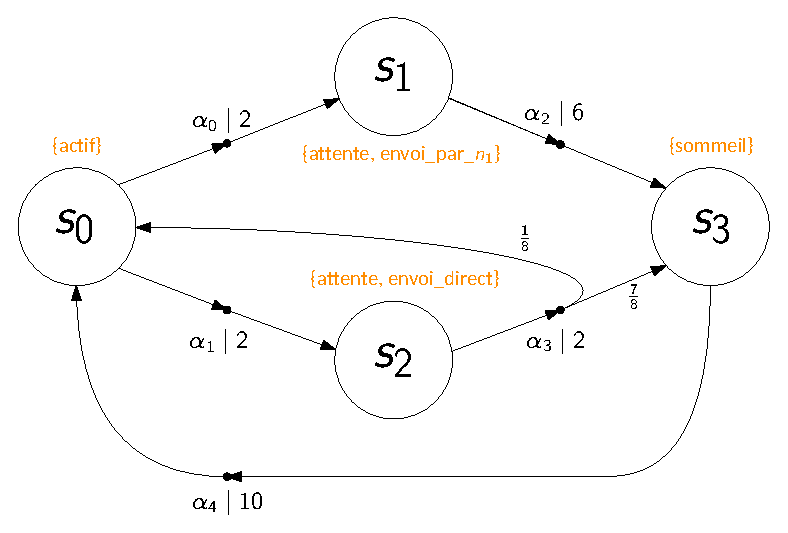
\includegraphics[width=\linewidth]{resources/main-mdp3}
      \end{column}
      \begin{column}{0.55\linewidth}\footnotesize
        \begin{itemize}
          \item Assurer un duty cycle de $12$ $ms$
          \item Bonne espérance pour atteindre {\color{DarkOrange}sommeil} en respectant ce duty cycle ?
        \end{itemize}
      \end{column}
    \end{columns}
\end{frame}

\begin{frame}{Bonne espérance sous un pire cas}{Algorithme}
  \vspace{-.1\linewidth}
  \begin{columns}
    \begin{column}{0.55\linewidth}
      \begin{enumerate}
        \item \textbf{\textit{\color{fibeamer@orange}Déplier}} $\mathcal{M}$ jusque $\ell_1$ depuis $s$
        \begin{itemize}
          \item[$\rightarrow$] jusque $12$ depuis $s_0$ ({\color{DarkOrange} actif})
        \end{itemize}
      \end{enumerate}
    \end{column}
    \begin{column}{0.45\linewidth}
      \begin{overprint}
        \onslide<1>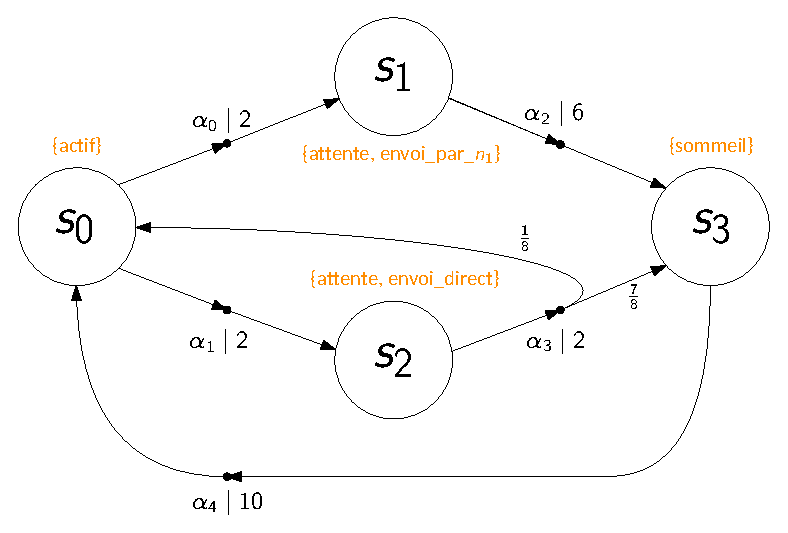
\includegraphics[width=\linewidth]{resources/main-mdp3}
        \onslide<2>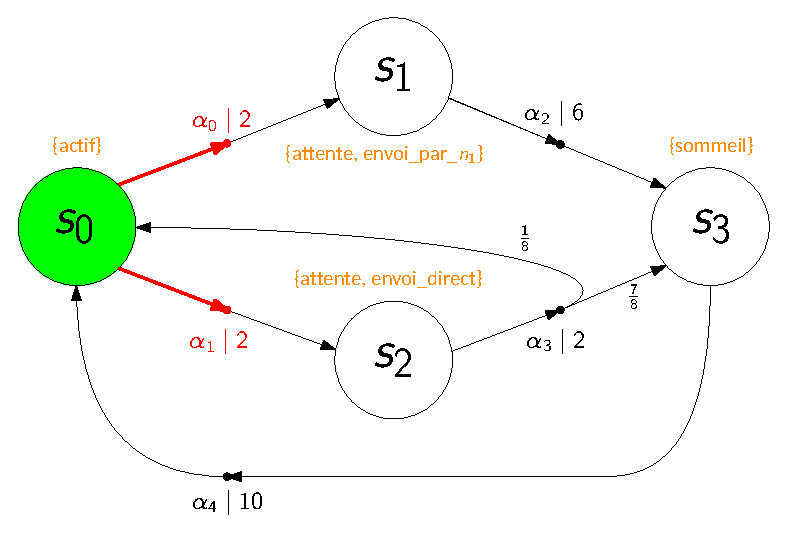
\includegraphics[width=\linewidth]{resources/unfold1_5}
        \onslide<3>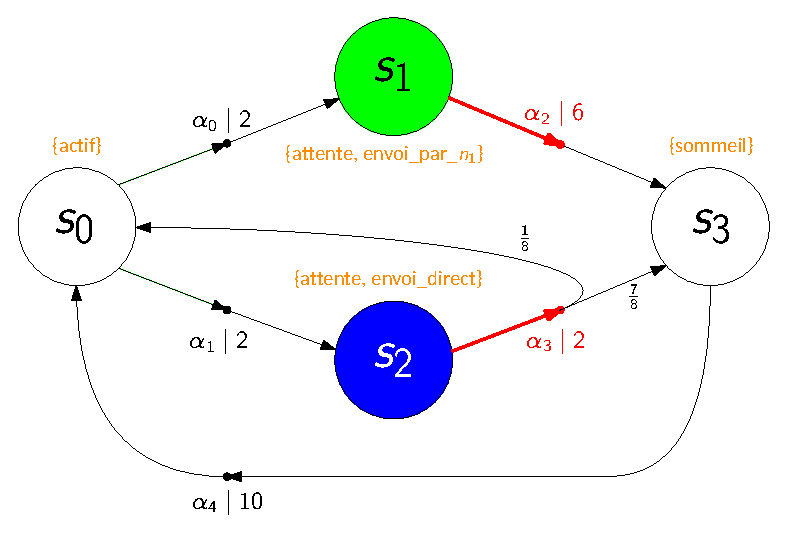
\includegraphics[width=\linewidth]{resources/unfold2_5}
        \onslide<4>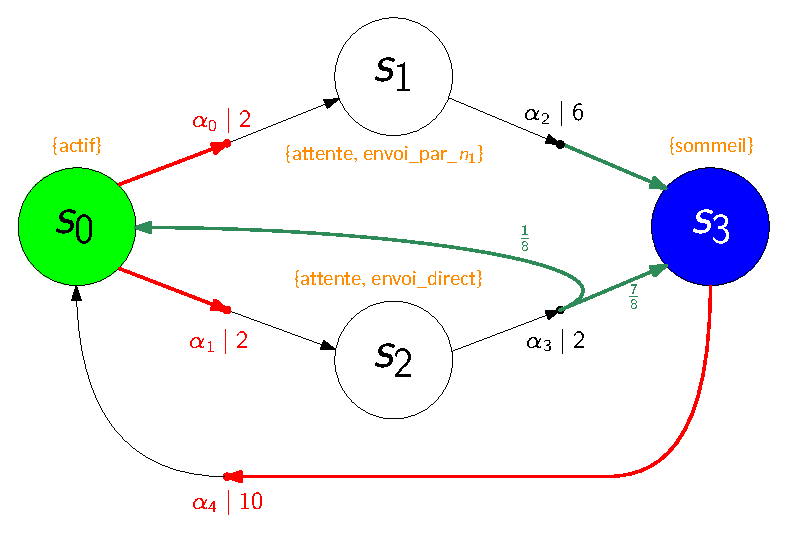
\includegraphics[width=\linewidth]{resources/unfold3_5}
        \onslide<5>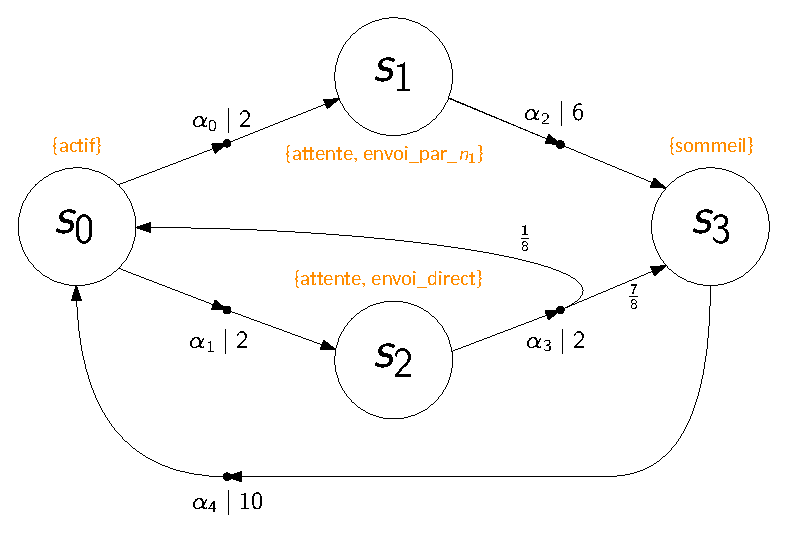
\includegraphics[width=\linewidth]{resources/main-mdp6}
      \end{overprint}
    \end{column}
  \end{columns}
  \begin{overprint}
    \onslide<2>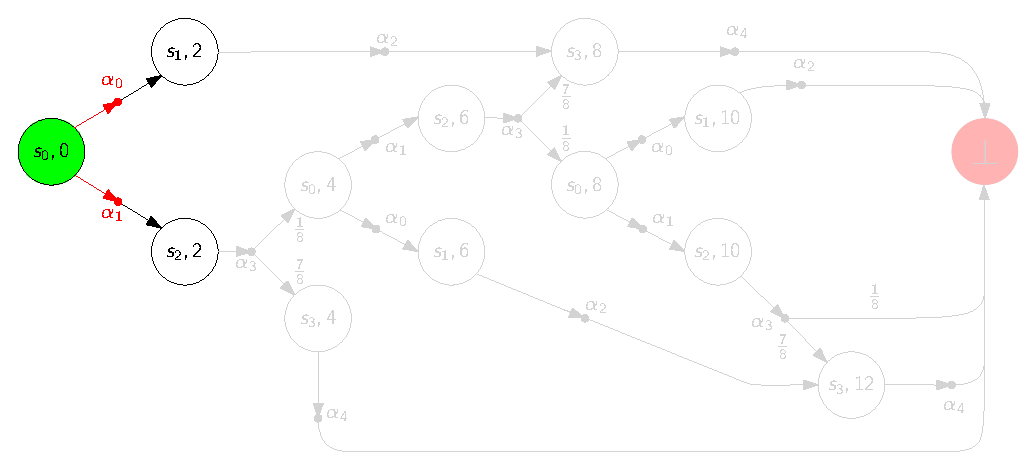
\includegraphics[width=\linewidth]{resources/unfold1}
    \onslide<3>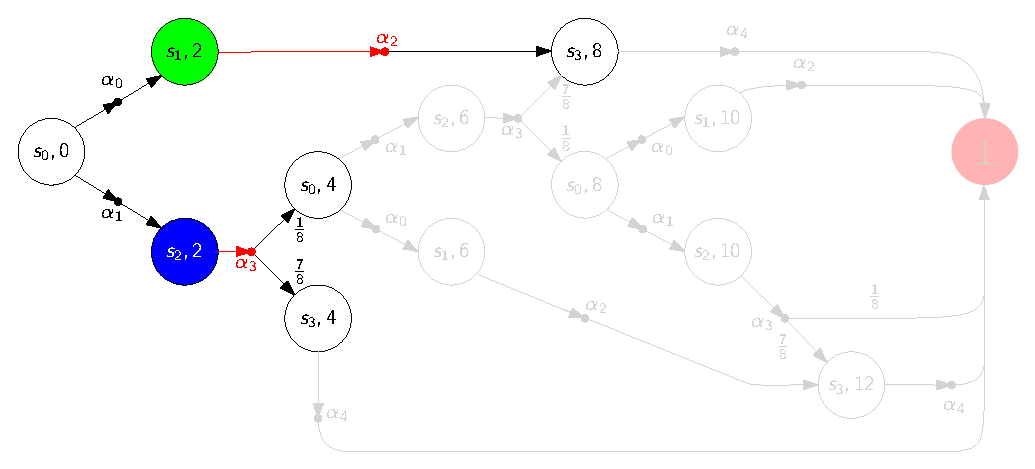
\includegraphics[width=\linewidth]{resources/unfold2}
    \onslide<4>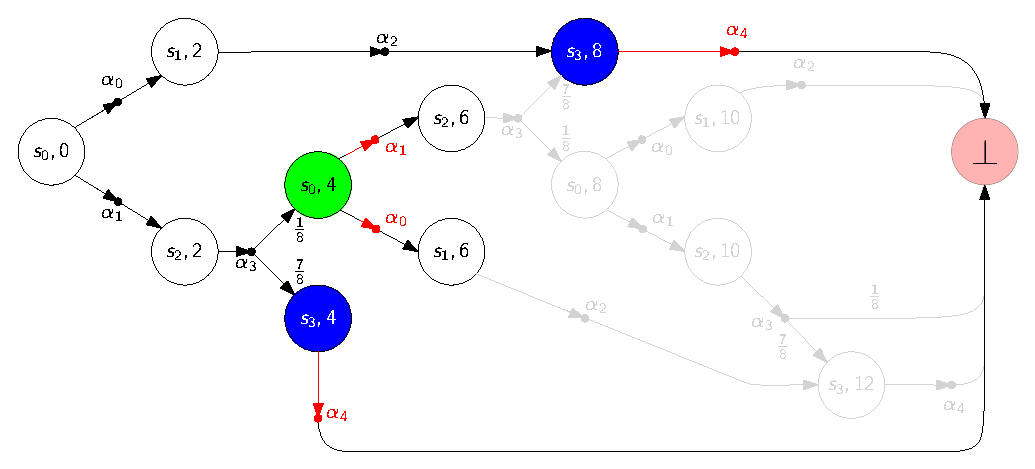
\includegraphics[width=\linewidth]{resources/unfold3}
    \onslide<5>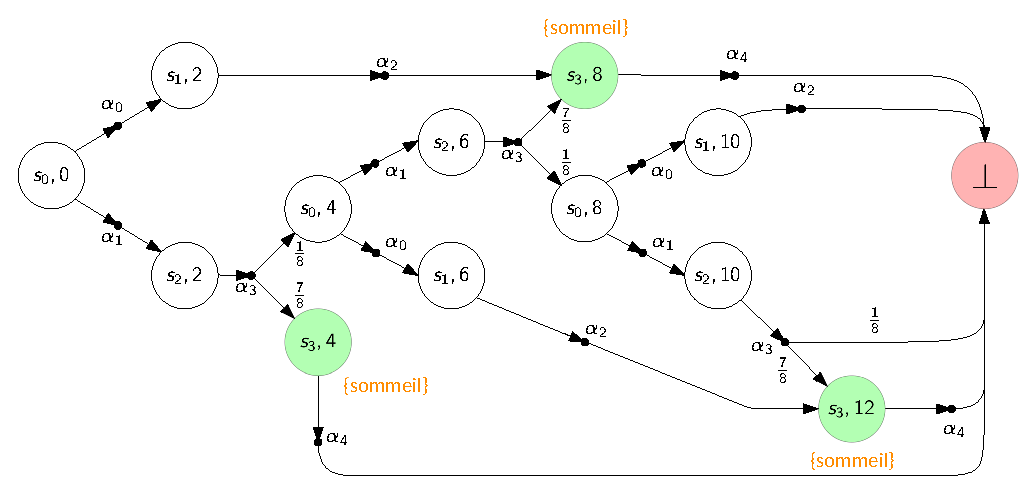
\includegraphics[width=\linewidth]{resources/example-unfolding}
  \end{overprint}
\end{frame}

% \begin{frame}{Bonne espérance sous un pire cas}{Algorithme}
% \begin{enumerate}
%   \item Déplier $\mathcal{M}$ jusque $\ell_1$ depuis $s$  $\color{fibeamer@blue} \leadsto $ $\color{fibeamer@blue}\mathcal{M}_{\ell_1}$
%   \item Calculer l'ensemble des actions \textit{\color{fibeamer@orange}safe} $\color{fibeamer@blue}\mathbb{A}$ de $\mathcal{M}_{\ell_1}$
%   \begin{itemize}
%     \item[$\leadsto$] on calcule les actions qui assurent au système d'atteindre les états cibles dans $\mathcal{M}_{\ell_1}$ quelle que soit l'évolution du système par l'incertitude liée aux probabilités
%   \end{itemize}
%   \item \textit{\color{fibeamer@orange}Limiter} l'espace d'action de $\mathcal{M}_{\ell_1}$ à $\mathbb{A}$ $\color{fibeamer@blue}\leadsto \mathcal{M}_{\ell_1}^\mathbb{A}$
%   \item Résoudre le problème du coût attendu jusqu'aux cibles dans $\mathcal{M}_{\ell_1}^\mathbb{A}$ $\color{fibeamer@blue}\leadsto ? \exists \sigma^*, \; \mathbb{E}^{\sigma^*}_{(s_0, 0)}(\TS^{\{(t, v) \; | \; t \in T \, \wedge \, v \leq \ell_1\}}) \leq \ell_2$
% \end{enumerate}

% \begin{itemize}
%   \item[$\rightarrow$]<2> Temps \textbf{\textit{\color{fibeamer@orange}pseudo-polynomial}} en la taille de $\color{fibeamer@blue}\ell_1$
%   \item[$\rightarrow$]<2> Stratégie à \textbf{\color{fibeamer@orange}mémoire pseudo-polynomiale}
% \end{itemize}
%
% \end{frame}

\begin{frame}{Bonne espérance sous un pire cas}{Algorithme}
    %\vspace{-.1\linewidth}
    \only<1>{
    \begin{enumerate}
      \item[1.] \textbf{\textit{\color{fibeamer@orange}Déplier}} $\mathcal{M}$ jusque $\ell_1$ {\color{fibeamer@blue}$\implies$} \alert{temps pseudo-polynomial en $\ell_1$}
    \end{enumerate}
    \[ ?{\exists} \sigma, \;
    \forall \pi \in Paths^{\sigma}(s), \, \TS^{\text{\color{DarkOrange} sommeil}}(\pi) \leq 12
    \wedge \mathbb{E}^{\sigma}_{s_0}(\TS^{\text{\color{DarkOrange} sommeil}}) \leq {\color{fibeamer@blue}6}
    \]
    }
    \only<2>{
    \begin{enumerate}
      \item[2.] Calculer l'ensemblde des actions \textbf{\textit{\color{fibeamer@orange}safe} $\color{fibeamer@blue}\mathbb{A}$} de $\mathcal{M}_{\ell_1}$
    \end{enumerate}
    \[ ?{\exists} \sigma, \;
    \forall \pi \in Paths^{\sigma}(s), \, \TS^{\text{\color{DarkOrange} sommeil}}(\pi) \leq 12
    \wedge \mathbb{E}^{\sigma}_{s_0}(\TS^{\text{\color{DarkOrange} sommeil}}) \leq {\color{fibeamer@blue}6}
    \]
    }
    \only<3>{
    \begin{enumerate}
      \item[3.] \textbf{\color{fibeamer@orange}\textit{Limiter}} le dépliage $\mathcal{M}_{\ell_1}$ aux actions \textbf{\textit{\color{fibeamer@orange}safe}} de $\mathbb{A}$ $\color{fibeamer@blue}\leadsto \mathcal{M}^\mathbb{A}_{\ell_1}$
    \end{enumerate}
      \[ \leadsto ? \exists \sigma^*, \; \mathbb{E}_{(s_0, 0)}^{\sigma*}(\TS^{\{ (s_3, v) \; | \; v \leq 12\}}) \leq 6\]
    }
    \only<4>{
      \begin{enumerate}
        \item[4.] {Résoudre le problème de bonne espérance jusqu'aux cibles dans $\color{fibeamer@blue}\mathcal{M}_{\ell_1}^\mathbb{A}$}
      \end{enumerate}
      \[ \leadsto \mathbb{E}_{(s_0, 0)}^{{\color{red}\sigma^*}}(\TS^{\{ (s_3, v) \; | \; v \leq 12\}}) = \frac{7}{8} \cdot 4 + \frac{1}{8} \cdot 12 = 5 \]
    }
    \begin{overprint}
      \onslide<1>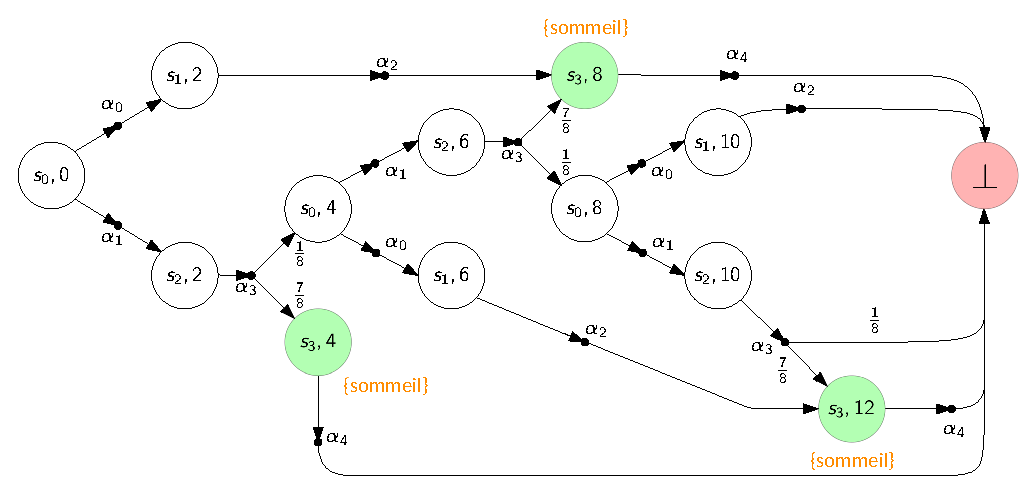
\includegraphics[width=\linewidth]{resources/example-unfolding}
      \onslide<2>
        \includegraphics[width=\linewidth]{resources/example-unfoldingA}
      \onslide<3>\includegraphics[width=0.95\linewidth]{resources/example-unfoldingA2}
      \onslide<4>\includegraphics[width=0.95\linewidth]{resources/example-unfoldingAnew}
    \end{overprint}
\end{frame}

\begin{frame}{Bonne espérance sous un pire cas}{Algorithme}\small
    \vspace{-.04\linewidth}
    \[
    \forall \pi \in Paths^{\color{fibeamer@orange}\sigma}(s), \, \TS^{\text{\color{DarkOrange} sommeil}}(\pi) \leq 12
    \wedge \mathbb{E}^{\color{fibeamer@orange}\sigma}_{s_0}(\TS^{\text{\color{DarkOrange} sommeil}}) \leq {6}
    \]
    \vspace{-.05\linewidth}
    \begin{columns}
    \begin{column}{0.5\linewidth}
    \begin{center}
      \includegraphics[width=\linewidth]{resources/example-unfoldingAnew}
    \end{center}
    \centering
    \footnotesize $\color{red}\sigma^*$ sans mémoire dans $\mathcal{M}_{12}^\mathbb{A}$
    \end{column}
    \begin{column}{0.5\linewidth}
    \begin{center}
      \includegraphics[width=\linewidth]{resources/main-mdp3}
    \end{center}
    \centering
      \footnotesize $\color{fibeamer@orange}\sigma$ à mémoire finie dans $\mathcal{M}$
    \end{column}
    \end{columns}
    \vspace{.02\linewidth}
    \begin{itemize}
      \item \textbf{\color{fibeamer@orange}Stratégie optimale $\sigma$} : tester une fois un envoi direct et passer par le noeud $n_1$ si l'envoi direct est un échec.
    \end{itemize}
\end{frame}

% \subsection{SSP-PQ}
%
% \begin{frame}{Poids à multiple dimensions} \small
%   \begin{itemize}
%     \item Supposons à présent que le poids de chaque action a $\color{fibeamer@blue}d$ dimensions
%   \[
%     \color{fibeamer@blue} w: A \rightarrow \mathbb{N}_0^d
%   \]
%     \vspace{-.07\linewidth}
%     \item[$\rightarrow$] ajout du coût en énergie
%   \end{itemize}
%   \begin{center}
%       \only<1>{\includegraphics[width=0.65\linewidth]{resources/mdpmdp}}
%       \only<2>{\includegraphics[width=0.65\linewidth]{resources/mdmdp2}}
%   \end{center}
% \end{frame}

% \begin{frame}{Requêtes percentiles dans les MDP multi-dimensionnels (SSP-PQ)}\footnotesize
%   %\textbf{\color{fibeamer@orange}Motivation} :
%   \begin{itemize}
%     \item \textbf{\color{fibeamer@blue}Requête percentile :} atteindre la cible avec un coût inférieur à un seuil $\color{fibeamer@blue}\ell \in \mathbb{N}_0$ et avec une probabilité supérieure à un seuil $\color{fibeamer@blue}\alpha \in [0, 1] \cap \mathbb{Q}$
%     \item[$\rightarrow$] satisfaire plusieurs requêtes percentiles \textbf{\textit{\color{fibeamer@orange}simultanément}} dans un MDP multidimensionnel
%   \end{itemize}
%   \begin{center}
%     \begin{columns}
%       \begin{column}{0.45\linewidth}
%         \includegraphics[width=\linewidth]{resources/mdpmdp2strat}
%       \end{column}
%       \begin{column}{0.55\linewidth}{\footnotesize
%         \begin{itemize}
%           \item $\mathcal{Q}_1 := \mathbb{P}^{\sigma_1}_{s_0}(\Diamond_{1\, :\, \leq 4} \; \text{\color{DarkOrange} sommeil}) \geq 0.8$
%           \item $\mathcal{Q}_2 := \mathbb{P}^{\sigma_2}_{s_0}(\Diamond_{2\, :\, \leq 700} \; \text{\color{DarkOrange} sommeil}) \geq 0.9$
%             \item[$\leadsto$] $\color{blue}\sigma_1 : $ envoi direct
%             \begin{itemize}\footnotesize
%               \item[$\implies$] \only<1>{$\mathbb{P}^{{\color{blue}\sigma_1}}_{s_0}(\Diamond_{1\, :\, \leq 4} \; \text{\color{DarkOrange} sommeil}) = 0.875$}
%               \only<2>{
%                 ne satisfait pas $\mathcal{Q}_2$
%               }
%             \end{itemize}
%             \item[$\leadsto$] $\color{red}\sigma_2 : $ envoi par un noeud intermédiaire
%             \begin{itemize}\footnotesize
%               \item[$\implies$] \only<1>{$\mathbb{P}^{{\color{red}\sigma_2}}_{s_0}(\Diamond_{2\, :\, \leq 700} \; \text{\color{DarkOrange} sommeil}) = 1$}
%               \only<2>{
%                 ne satisfait pas $\mathcal{Q}_1$
%               }
%           \end{itemize}
%         \end{itemize}
%         }
%       \end{column}
%     \end{columns}
%   \end{center}
% \end{frame}


% \begin{frame}{Requêtes percentiles dans les MDP multi-dimensionnels (SSP-PQ)}\small
%   %\textbf{\color{fibeamer@orange}Motivation} :
%   \begin{itemize}
%     \item \textbf{\color{fibeamer@blue}Requête percentile :} atteindre la cible avec un coût inférieur à un seuil $\color{fibeamer@blue}\ell \in \mathbb{N}_0$ et avec une probabilité supérieure à un seuil $\color{fibeamer@blue}\alpha \in [0, 1] \cap \mathbb{Q}$
%     \item[$\rightarrow$] satisfaire plusieurs requêtes percentiles \textbf{\textit{\color{fibeamer@orange}simultanément}} dans un MDP multidimensionnel
%   \end{itemize}
%   \begin{center}
%     \begin{columns}
%       \begin{column}{0.45\linewidth}
%         \includegraphics[width=\linewidth]{resources/mdmdp2}
%       \end{column}
%       \begin{column}{0.55\linewidth}\footnotesize
%         \begin{itemize}
%           \item $\mathcal{Q}_1 := \mathbb{P}^{\sigma}_{s_0}(\Diamond_{1\, :\, \leq 4} \; \text{\color{DarkOrange} sommeil}) \geq 0.8$
%           \item $\mathcal{Q}_2 := \mathbb{P}^{\sigma}_{s_0}(\Diamond_{2\, :\, \leq 700} \; \text{\color{DarkOrange} sommeil}) \geq 0.9$
%         \end{itemize}
%       \end{column}
%     \end{columns}
%   \end{center}
% \end{frame}


% \begin{frame}{Requêtes percentiles dans les MDP multi-dimensionnels (SSP-PQ)}\small
%       $\sigma_{1 \wedge 2} := $ essayer une fois un envoi direct et passer ensuite par $n_1$ si l'envoi direct a échoué
%   \begin{center}
%     \begin{columns}
%       \begin{column}{0.45\linewidth}
%         \includegraphics[width=\linewidth]{resources/mdmdp2}
%       \end{column}
%       \begin{column}{0.55\linewidth}{ \scriptsize
%         \begin{itemize}
%           \item $\mathcal{Q}_1 := \mathbb{P}^{\sigma_{1 \wedge 2}}_{s_0}(\Diamond_{1\, :\, \leq 4} \; \text{\color{DarkOrange} sommeil}) \geq 0.8$
%           \item $\mathcal{Q}_2 := \mathbb{P}^{\sigma_{1 \wedge 2}}_{s_0}(\Diamond_{2\, :\, \leq 700} \; \text{\color{DarkOrange} sommeil}) \geq 0.9$
%           \item $\mathbb{P}^{\sigma_{1 \wedge 2}}_{s_0}(\Diamond_{1\, :\, \leq 4} \; \text{\color{DarkOrange} sommeil}) = 0.875 \models \mathcal{Q}_1$
%           \item $\mathbb{P}^{\sigma_{1 \wedge 2}}_{s_0}(\Diamond_{2\, :\, \leq 700} \; \text{\color{DarkOrange} sommeil}) = 1 \models \mathcal{Q}_2 $
%           \begin{itemize}
%             \scriptsize
%             \item[$\leadsto$] $394 \leq \TS^{\text{\color{DarkOrange} sommeil}}(\pi) \leq 690$ $\forall \pi \in Paths^{\sigma_{1 \wedge 2}}(s_0)$
%           \end{itemize}
%         \end{itemize}
%         }
%       \end{column}
%       \end{columns}
%       \end{center}
% \end{frame}

% \begin{frame}{SSP-PQ : résolution du problème}\footnotesize
%   \vspace{-.02\linewidth}
%   \begin{itemize}
%     \item Requiert un \textbf{\color{orange}dépliage} sur \textbf{\color{fibeamer@orange}toutes les dimensions} jusqu'au coût le plus élevé $\color{fibeamer@blue}\ell$
%     \begin{center}
%     \includegraphics[width=0.8\linewidth]{resources/SSP-PQ-unfolding}
%     \end{center}
%     \item[$\implies$] $S_{\ell} = S \times \{0, \dots, \ell \}^d$
%     \item[$\implies$] Temps \textbf{\color{fibeamer@orange} exponentiel}% en $\color{fibeamer@blue}d$
%     \item Satisfaire le problème $\implies$ stratégies \textbf{\color{fibeamer@orange}randomisées} à \textbf{\color{fibeamer@orange}mémoire exponentielle}
%     \item \alert{Il n'y a pas une stratégie optimale} $\color{fibeamer@blue}\rightarrow$ compromis entre les $\color{fibeamer@blue}q$ requêtes
%     \item On ne peut pas améliorer une solution d'une requête sans dégrader la solution d'une autre requête
%   \end{itemize}
% \end{frame}

\section{Résultats et perspectives}
\begin{frame}{Résultats}
\begin{scriptsize}
\begin{tabular}{|c|c|c|c|}
\hline
\textbf{Problème}                                                                                                     & \textbf{Temps}                                   & \multicolumn{2}{c|}{\textbf{Stratégie}} \\ \cline{3-4}
                                                                                                                      &                                                  & \textit{type}     & \textit{mémoire}    \\ \hline
 SR (accessibilité)                                                                                                    & P($\mathcal{M}$)                                 & pure              & sans mémoire        \\ \hline
 \textbf{\color{fibeamer@orange}SSP-E (bon coût moyen attendu)}                                                                                                  & \textbf{\color{fibeamer@orange}P($\mathcal{M}$)}                                 & \textbf{\color{fibeamer@orange}pure}              & \textbf{\color{fibeamer@orange}sans mémoire}        \\ \hline
 SSP-P (requête percentile)                                                                                            & P($\mathcal{M}$) $\cdot$ P$_{ps}$($\ell$)        & pure              & P$_{ps}$($\ell$)    \\ \hline
SP-G  (garantie de coût)                                                                                              & P($\mathcal{M}$)                                 & pure              & sans mémoire        \\ \hhline{|=|=|=|=|}
{\bfseries \color{fibeamer@orange}SSP-WE (garantie + bonne espérance)}                                                                                   & {\bfseries \color{fibeamer@orange}P($\mathcal{M}$) $\cdot$ P$_{ps}$($\ell$)}        & {\bfseries \color{fibeamer@orange} pure}              &      {\bfseries \color{fibeamer@orange}P$_{ps}$($\ell$)}    \\ \hline
\begin{tabular}[c]{@{}c@{}}MOSR\\ (accessibilité multiple\\ + états cibles absorbants)\end{tabular} & P($\mathcal{M}$)                                 & randomisée        & sans mémoire        \\ \hline
MOSR (accessibilité multiple)                                                                                         & P($\mathcal{M}$) $\cdot$ E($\mathcal{Q}$)        & randomisée        & E($\mathcal{Q}$)    \\ \hline
\begin{tabular}[c]{@{}c@{}}SSP-PQ\\ (Multiple requêtes percentiles\\ sur une seule dimension)\end{tabular}            & P($\mathcal{M}$) $\cdot$ P$_{ps}$($\ell_{\max}$) & randomisée        & P$_{ps}$($\ell$)    \\ \hline
\begin{tabular}[c]{@{}c@{}}SSP-PQ\\ (Multiples requêtes percentiles\\ sur multiple dimensions)\end{tabular}           & P($\mathcal{M}$) $\cdot$ E($\mathcal{Q}$)        & randomisée        & E($\mathcal{Q}$)    \\ \hline
\end{tabular}
\captionof{table}{$P$ : polynomial -- $P_{ps}$ : pseudo-polynomial -- $E$ : exponentiel}
\end{scriptsize}
\footnotesize
\end{frame}

\begin{frame}{Perspectives}
\begin{itemize}
  \item \textbf{\color{fibeamer@orange}Problème d'explosion de l'espace d'état} : abstraction du système en utilisant les jeux stochastiques, exploration de l'espace d'état par machine learning
  \item \textbf{\color{fibeamer@orange}Stratégies compréhensibles} : stratégies ``moins optimales'' mais sans aléatoire
  \item \textbf{\color{fibeamer@orange}Pas de dépliage}
  \item \textbf{\color{orange}Autres fonctions de coût} : mean-payoff, discounted sum, etc.
  \item[$\rightarrow$] Implémentation de nouveaux algorithmes dans \sfont{\color{fibeamer@orange}Storm}
\end{itemize}
\end{frame}

% \subsection{}
% \begin{frame}[allowframebreaks]
%         \nocite{*}
%         \frametitle{Références}
%       \printbibliography
% \end{frame}

\end{document}
